%*******************************************************************************
%****************************** Second Chapter *********************************
%*******************************************************************************

\chapter{Exercise Knowledge Point Mining Based on Graph Neural Network}

\ifpdf
    \graphicspath{{Chapter2/Figs/Raster/}{Chapter2/Figs/PDF/}{Chapter2/Figs/}}
\else
    \graphicspath{{Chapter2/Figs/Vector/}{Chapter2/Figs/PDF/}{Chapter2/Figs/}}
\fi


\section{Research Motivation}
%在推荐系统的各环节,包括数据收集、数据挖掘和数据推荐,都以建立高质量的数据集作为基础。对于本文的研究主题习题推荐系统而言,建立一个规范的习题库对于建立一个试题推荐系统是重要的第一步。题库建设也是一项十分复杂而困难的工作,需要综合考虑习题数据的各个层面,为习题添加足够多的附加信息用于后续的数据挖掘。高中数学具有数百个知识点,平均每个知识点有从易到难的不同难度梯度的数十道习题。一个优质数学学科题库的规模为十万规模。除去数量上的要求,优质题库除了题目质量,以及对教育内容(教材)的匹配度之外,还有两个根本性问题,其一为知识点关系网络构建,其二为知识点-习题关系构建。而就是对于这些因素的优化,导致了优质题库的建设门槛,以及极高的成本。而市面上的题库往往缺失了对于这些因素的重视,导致出现了许多质量不高的习题数据库。所以,对题目的知识点标签的标注,以及知识体系的构建,是优质题库建设过程中最为核心的问题之一。

In this thesis's study topic, establishing a high-quality data source is the critical step of building the recommendation system. The construction of an exercise corpus is a complex and challenging task, requiring consideration of all aspects of the exercise data and adding enough additional information to subsequent data mining exercises. High school mathematics has hundreds of knowledge points, and on average, each point has dozens of exercises of different difficulty gradients from easy to difficult. The size of a high-quality math subject exercise corpus is 100,000 scale. In addition to the quantitative requirements, there are two fundamental issues in a quality exercise corpus, in addition to the quality of the questions and the matching of the educational content, one is the construction of the knowledge point relationship network, and the other is the construction of the knowledge point-exercise relationship.

Moreover, it is the optimization of these factors that leads to the construction of a high-quality exercise corpus and the extremely high cost. The question databases on the market often lack attention to these factors, leading to the emergence of many poor-quality exercise databases. Therefore, labeling the questions' knowledge points and constructing the knowledge system is one of the most critical issues in building a quality exercise corpus.

%建立试题推荐系统的一个关键问题是如何结合知识点来推荐题目。在考虑这个问题的解决方案的时候,我们首先要考虑的是,我们需要什么样的知识体系和知识点标签。在教材和教学大纲中,以及各种教辅中,会有各种对``知识点''的描述。在高中数学中的知识点,如函数、定义域、值域或解析式等,有直接的概念,也有方法的应用,有专题的抽象,也有相似解法的汇总。这并没有一种标准的分类方法,知识点系统构建的方法可能是千差万别的。作为数据挖掘的任务而言,我们更关注其涉及到的概念和技能点,这些可以通过习题文本来进行隐藏信息挖掘。作为一个对学生知识掌握熟练度进行分析的习题推荐系统,那么知识点的标签应该要能够描述题目测验的核心知识点、方法或思路,要能够区分对于学生的能力要求点,这样才能构建更为强大的用户知识点掌握度模型和推荐引擎。

One of the critical problems in building a test recommendation system is recommending topics in conjunction with knowledge points. When referring to the solution to this problem, the knowledge point labels should be considered. In textbooks and syllabi and various teaching aids, there are various descriptions of ``knowledge points''. Knowledge points in high school mathematics, such as functions, definition domains, value domains, or analytic equations, have direct concepts, applications of methods, abstractions of topics, and summaries of similar solutions. There is no one standard way to classify these, and the methods of knowledge point system construction may be very different. As far as the task of data mining is concerned, this thesis is more concerned with the concepts and skill points it involves, and these can be concluded for confidential information through the text of the exercises. As an exercise recommendation system that analyzes students' knowledge mastery proficiency, the knowledge point labels should be able to describe the core knowledge points, methods, or ideas of the topic quiz and be able to distinguish the ability requirement points for students to build a more robust user knowledge mastery model and recommendation engine.
%在本章中,挖掘的知识点标签,是用于题目的推荐和分析报告。它要求完善题目的知识点关联,即对题目打上若干对应的知识点标签,其中知识点之间也会存在依赖关系,另外就是要建立完整的知识点知识图谱用于生成学生的学习报告。对于第一个问题,它实际上是用题目文本来进行知识点挖掘的任务,也是一个分类任务。具体一点而言,主要是依据题目短文本信息进行层次化分类的任务。在这个任务中,我们需要使用到最基础的技术是自然语言处理和机器学习。也即,通过对大量人工标注好的题目文本和知识点标签结果(也称为训练语料)的学习——通过自然语言处理的技术获取题目文本的特征,通过机器学习来得到分类模型——从而使得系统具有了自动做知识点分类的能力。在这个定义中,待分类对象为题目(包括题干、答案、解析等等),分类结果是一组知识点标签。学习系统的输入就是一组训练习题,即\(n\)道已经标注好的题目及其对应的知识点标签;学习系统依据训练数据,训练给定的分类模型。在预测阶段,输入待标注的习题,输出一组对习题知识点的预测标注结果。

\section{Research Contribution}
%本章提出了一种习题的多知识点标签分类方法,它利用习题的题目描述的文本信息来识别习题相关的知识点,本质上是一种文本分类任务。提出的方法分为利用基于注意力机制的双向LSTM文本信息表征网络和基于图卷积网络传播机制的多知识点标签分类器生成网络两个部分。在文本信息表征网络中,习题和知识点文本都是作为输入向量,输出的习题文本作为最终的习题信息表征。而知识点文本向量则进一步在标签生成器网络中进行图卷积网络传播学习,以嵌入知识点间的相互关系,最终习题表征向量与输出的知识点分类进行乘积计算来获取习题的知识点标签。

%本章的主要创新点在于用图网络的节点信息传播机制来表征学习知识点间的关系。从而让模型可以通过较容易分类的知识点联想到隐藏的相关知识点。

This chapter's main contribution is the relationships between knowledge points with graph networks' node information propagation mechanism, enabling the model to associate hidden related knowledge points through the tagged classified knowledge points. A multi-knowledge point label classification method for exercises is proposed, which uses the textual information described by the exercise text to identify the knowledge points related to the exercise, essentially a text classification task. The proposed method is divided into two parts: a bidirectional LSTM textual information representation network with attention mechanism and a multi-knowledge point labeled classifier generation network based on a graph convolutional network propagation mechanism. In the text information representation network, both the exercise and knowledge point texts are input vectors, and the output exercise text is used as the final exercise information representation. Subsequently, the knowledge point text vector is further learned by graph convolutional network propagation in the label generator network to embed the interrelationships among knowledge points. The final exercise representation vector is calculated by multiplying with the output knowledge point classification to obtain the exercises' knowledge point labels. After experimental validation, the proposed model outperforms the original DKVMN and other baseline models in the proposed metrics.


% This chapter proposed a multi-knowledge point label classification method for exercises, which uses the textual information described by the title of the exercise to identify the knowledge points related to the exercise, essentially a text classification task. The proposed method is divided into two parts: a bidirectional LSTM textual information representation network using an attention-based mechanism and a multi-knowledge point labeled classifier generation network based on a graph convolutional network propagation mechanism. Both the exercises and labels utilize textual information as representations, and they are generated through the text module.

%本章提出了一种习题的多知识点标签分类方法。该方法分为利用Attentional双向LSTM进行文本信息表征模块和基于GCN网络传播机制的多知识点标签分类器生成模块两个部分。习题和标签都利用文本信息来作为表征,它们通过文本模块来生成。

%In this chapter, a multi-knowledge point label classification method for exercises is proposed. The method is divided into two parts: a text information characterization module using Attentional bidirectional LSTM and a multi-knowledge point labeling classifier generation module based on the GCN network propagation mechanism. Both exercises and labels utilize textual information as representations,which are generated through the text representation module.


%文本部分利用分类器对习题进行知识点标注任务。挖掘出的知识点标签用于题目推荐和分析报告。它需要提炼题目的知识点关联,即为题目提供若干对应的知识点标签。知识点之间也会存在依赖关系,建立完整的知识点知识图谱,用于生成学生学习报告。第一个问题是利用主题文本进行知识点挖掘任务,也是一个分类任务。更具体地说,它是一个基于话题短文信息的分层分类任务。在这个任务中应该使用最基本的自然语言处理(NLP)技术和机器学习。通过学习大量人工标注的话题文本和知识点标注结果(也叫训练语料)--通过NLP技术获得话题文本的特征,通过机器学习获得分类模型。系统可以自动进行知识点分类。在这个定义中,待分类的对象是一个话题(包括题干、答案、释义等),结果是一组知识点标签。学习系统的输入是一组训练练习,即已被贴上相应知识标签的问题;学习系统根据训练数据对给定的分类模型进行训练。在预测阶段,利用习题输入的待标签,输出一组习题知识点的预测标签结果。

%本章提出了一种习题的多知识点标签分类方法。该方法分为利用Attentional双向LSTM进行文本信息表征和利用GCN嵌入学习法生成多知识点标签分类器。最后,利用分类器对习题进行知识点标注任务。挖掘出的知识点标签用于题目推荐和分析报告。它需要提炼题目的知识点关联,即为题目提供若干对应的知识点标签。知识点之间也会存在依赖关系,建立完整的知识点知识图谱,用于生成学生学习报告。第一个问题是利用主题文本进行知识点挖掘任务,也是一个分类任务。更具体地说,它是一个基于话题短文信息的分层分类任务。在这个任务中应该使用最基本的自然语言处理(NLP)技术和机器学习。通过学习大量人工标注的话题文本和知识点标注结果(也叫训练语料)--通过NLP技术获得话题文本的特征,通过机器学习获得分类模型。系统可以自动进行知识点分类。在这个定义中,待分类的对象是一个话题(包括题干、答案、释义等),结果是一组知识点标签。学习系统的输入是一组训练练习,即已被贴上相应知识标签的问题;学习系统根据训练数据对给定的分类模型进行训练。在预测阶段,利用习题输入的待标签,输出一组习题知识点的预测标签结果。


\section{Proposed Model}
In this chapter, a multi-knowledge point labeling classification method for exercises is proposed. The method is divided into textual information characterization using Attention-based bidirectional LSTM and multi-knowledge point labeling classifier generation using the GCN embedding learning method. Finally, the classifier is used to perform the knowledge point labeling tasks on the exercises. The knowledge point labels are mined for topic recommendation and analysis reports. It requires refining the topic's knowledge point association, i.e., several corresponding knowledge point tags for the topic. There will also be dependencies between the knowledge points and build a complete knowledge map of knowledge points for generating student learning reports. The first problem is a knowledge point mining task using the topic text, which is also a classification task. To be more specific, it is a hierarchical classification task based on the topic's short text information. The most basic natural language processing (NLP) technologies and machine learning should be used in this task. By learning a large amount of manually labeled topic text and knowledge point labeling results (also called training corpus) - obtaining the features of the topic text through NLP techniques and obtaining the classification model through machine learning. The system can do knowledge point classification automatically. The object to be classified is a topic (including stem, answer, paraphrase, etc.), and the result is a set of knowledge point labels. The input to the learning system is a set of training exercises, i.e., \(n\) questions that have been labeled with their corresponding knowledge labels; the learning system trains the given classification model based on the training data. In the prediction phase, the exercises' input to be labeled is used to output a set of predicted labeling results for the exercises' knowledge points.


% In this section, a graph neural network-based model is proposed for test question-knowledge point association and knowledge mapping of knowledge points. The architecture has two segments. The first one is an exercise-knowledge point association module implemented with a semi-supervised learning algorithm based on GCNs and text mining embedding learning for test knowledge point labeling and association. The second part considers the systematization of high school mathematics knowledge and combines a priori domain knowledge with an improved R-GCN algorithm to construct a knowledge graph of high school mathematics knowledge points.

\subsection{Algorithm Overview}
%本节的任务是构造一个挖掘习题-知识点关系的模型和一个挖掘知识点之间关联的模型。建立习题-知识点关系即对习题进行知识点标注,习题的知识点是理解习题和求解习题所用到的知识概念的集合。所以准确描述一道试题的知识点,对于后续的知识追踪和推荐过程十分重要。目前已经存在的基础分类方式有专家标注和机器学习两种方式。前者即教育专家结合自己的专业知识对试题进行知识点标注,但当题量或题目复杂度较高时,人工标注存在工作量大,主观度高和标注不完善等问题。另外考虑到知识点之间的关联,人工标注也存在无法考虑到知识内联关系。另一种方式则是用基于规则的自动化标注的方法,它通过文本模式匹配等非智能方式来进行知识点关键词匹配。但有许多习题往往并不具有显式的知识点文本,因此该方法的正确率不够理想。此外,一个习题往往具有多个知识点,因此实际上知识点挖掘是一个多标签分类问题~\cite{tsoumakas2007multi,zhang2013review,liu2020emerging}。本章也会对``如何有效建模知识点间的关系''来进行讨论并提出一种基于图神经网络的多标签分类模型。

This section aims to construct a model for mining the exercise-knowledge point relationship and mining the association between knowledge points. Establishing an exercise-knowledge point relationship means labeling the knowledge points of an exercise and collecting knowledge concepts to understand and solve the exercise. Therefore, accurately describing a test question's knowledge points is essential for the subsequent knowledge tracing and recommendation process. The two basic classification approaches that already exist are expert labeling and machine learning. The former means that education experts combine their professional knowledge to label knowledge points of test questions. However, when the number of questions or complexity of questions is high, manual labeling has a high workload, high subjectivity, and imperfect labeling. Also, considering the association between knowledge points, the manual labeling has the problem of not taking into account the inline knowledge relationship. Another way is to use the rule-based automated labeling method, which performs knowledge keyword matching by non-intelligent means such as text pattern matching. However, many exercises often do not have explicit knowledge point texts, so this correctness rate is not satisfactory. Also, an exercise often has multiple knowledge points, so in effect, knowledge point mining is a multi-label classification problem~\cite{tsoumakas2007multi,zhang2013review,liu2020emerging}. This chapter also discusses ``how to effectively model the relationships between knowledge points'' and proposes a multi-label classification model based on graph neural networks.


%在2019年,提出了一种多标签图像分类模型,受该模型启发,本章提出了一个基于注意力机制习题文本特征提取和基于图神经网络知识点关系挖掘的多知识点标注模型,它通过数据驱动的方式建立知识点关系图描述知识点间的关联关系,对知识点分别建立分类器,然后对习题的文本特征进行多标签分类。其主要架构图如下。

In 2019, a multi-label image classification model was proposed~\cite{chen2019multi}. Inspired by this model, this chapter proposes a multi-knowledge point labeling model based on attention mechanism exercise description text feature extraction and graph convolutional neural network (GCN) based knowledge point relationship mining, which builds a knowledge point relationship graph to describe the association relationship between knowledge points by a data-driven approach, builds classifiers for knowledge points separately, and then performs multi-label classification. Its main architecture diagram is shown in \figname{\ref{fig:ch2-modelarchitecture}}.

\begin{figure}[htb]
    \centering
    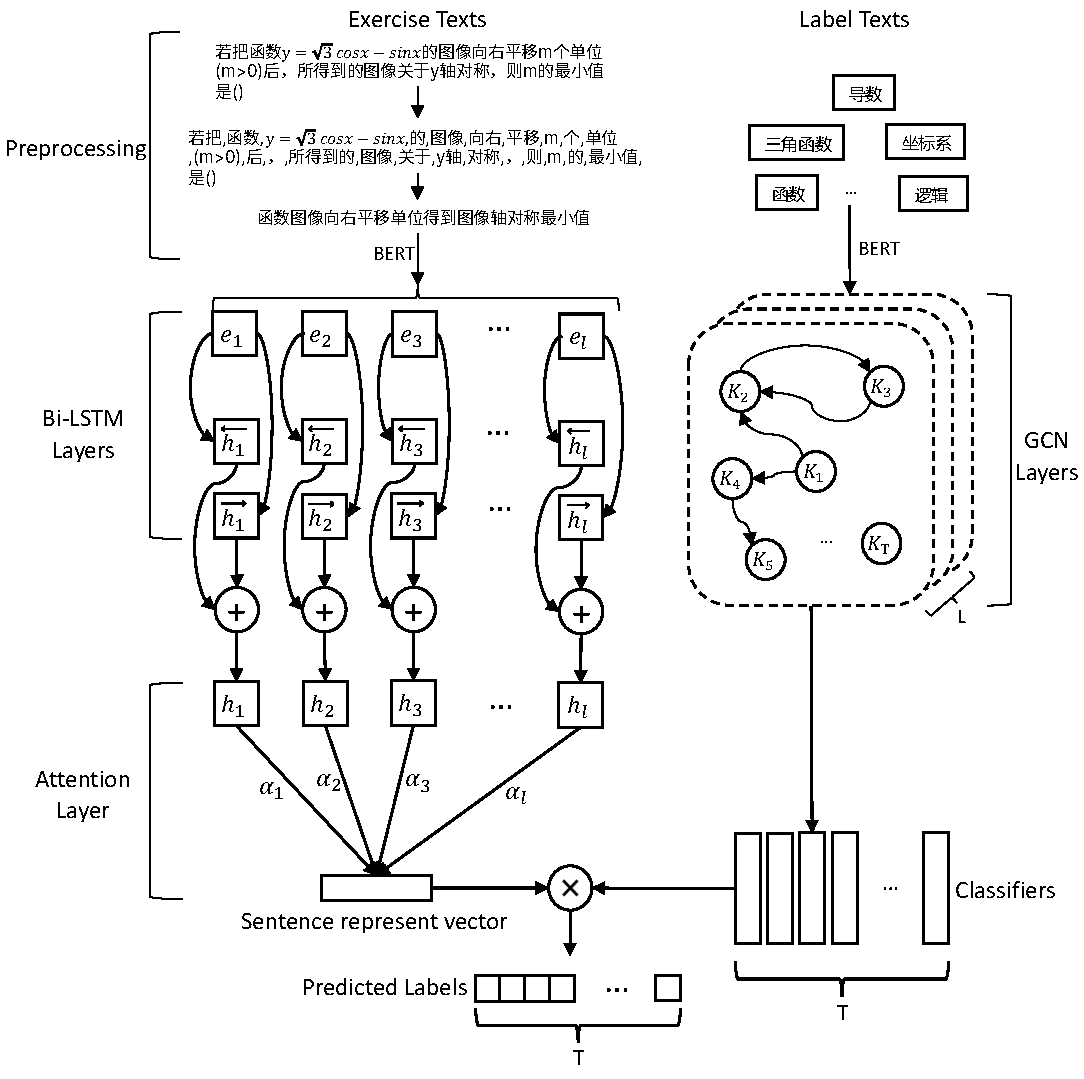
\includegraphics[width=1.0\textwidth]{ch2-ov.pdf}
    \caption{Structure of the knowledge labeling model}\label{fig:ch2-modelarchitecture}
\end{figure}

%从结构上我们可以看到,模型中一般有两部分,其中

%第一部分是习题文本挖掘模块 ,它用自然语言处理技术来对题目(包括问题描述和答案)进行文本挖掘,它包含隐藏的知识点信息。本文设计了一个端到端的网络训练方式,实现模型整体的迭代学习。具体而言,它包括进行文本分词、过滤和去重登部分的文本预处理部分,进行词向量embedding计算的embedding层和进行文本信息挖掘的基于Attention的双向LSTM网络,该网络由Peng等人于2016年提出~\cite{zhou2016attention},输出一个对于习题文本的向量表示。

%第二部分是基于图卷积神经网络的知识点关联多标签分类器,它将知识点映射到一组相互依赖的目标分类器。这些分类器与第一部分输出的习题信息表征向量进行计算,输出一个代表各个知识点标注概率的结果向量。

From the structure, it can be seen that there are generally two parts to the model:
\begin{enumerate}
    \item The first part is the exercise description text information mining module, which uses a Bi-LSTM network with an added attention mechanism to text-mine hidden knowledge information on questions (including question descriptions and answers). In this thesis, an end-to-end network training approach is designed to achieve the model's overall iterative learning. Specifically, it consists of a text preprocessing part that performs the text subdivision, filtering, and deduplication parts, an embedding layer that performs the word vector embedding calculation, and an Attention-based Bi-LSTM (Bi-LSTM) network that performs text information mining, which was proposed by Peng et al.\ in 2016~\cite{zhou2016attention}, outputting a textual information representation vector.
    \item The second part is a GCN-based knowledge point association multi-label classifier, which maps knowledge points to a set of interdependent target classifiers. These classifiers are multiplied with the exercise information representation vector outputted by the first part to output a result vector representing each knowledge point's labeling probability.
\end{enumerate}


\subsection{The Exercise Description Text Mining}
%本部分基于Peng等人提出的Attention based Bi-LSTM模型,该模型的结构如图所示\ref{}
This section is based on the attention-based Bi-LSTM, including four layers: Preprocess Layer, Embedding Layer, Bi-LSTM layer, Attention Layer, and Output Layer:
\subsubsection{Pre-process Layer}

%在预处理阶段,主要包括分词、清洗、正则化等方式。考虑到我们的研究对象为中文高中数学试题,相对于英文,中文句子中间没有中间空格,所以必须用分词算法来将句子分解为分词。内容中有很多对句意表达无关的文本,如果直接进行计算会造成大量的干扰和冗余信息,所以另外的文本清理也是必要的步骤。\figname{ref{ch2-fig3}}显示了一个预处理练习文本的例子。

% - 中文分词是中文自然语言处理的一个基本步骤,在中文中,一个句子中词与词之间没有自然分隔,因此必须先对句子进行分词操作,将句子分解为词。分词效果将直接影响词性、句法树等模块的效果。选择合适的的中文分词算法能够达到更好的自然语言处理效果,帮助计算机理解复杂的中文语言。目前,中文分词主要分为基于词典规则匹配和基于统计模型两种算法,相对于前者,后者具有更好的泛化性和学习能力,对先验规则之外的分词例如歧义词和未登录词表现更好。在本模型中,采用了目前较为热门的jieba分词器,它采用了基于汉字成词能力的 HMM 模型,能够找出基于词频的最大切分组合。用户也可以自定义停用词和用户词典来实现对于专有名词的识别。

% - 清洗:在对习题进行文本挖掘时,会遇到大量无关的文本信息,例如对于以下习题:

The preprocessing stage mainly includes word separation, cleaning, and regularization. Considering that our research object is Chinese high school mathematics test questions, compared with English, there is no middle space in the middle of sentences of Chinese language, so it is necessary to use the word separation algorithm to decompose the sentences into subwords. There are many texts in the content that are irrelevant to the sentence expression, which will cause much interference and redundant information if the calculation is performed directly, so additional text cleaning is also a necessary step. The \figname{\ref{fig:ch2-model-preprocessing}} shows an example of preprocessing of an exercise description text.

\begin{figure}[htbp!]
    \centering
    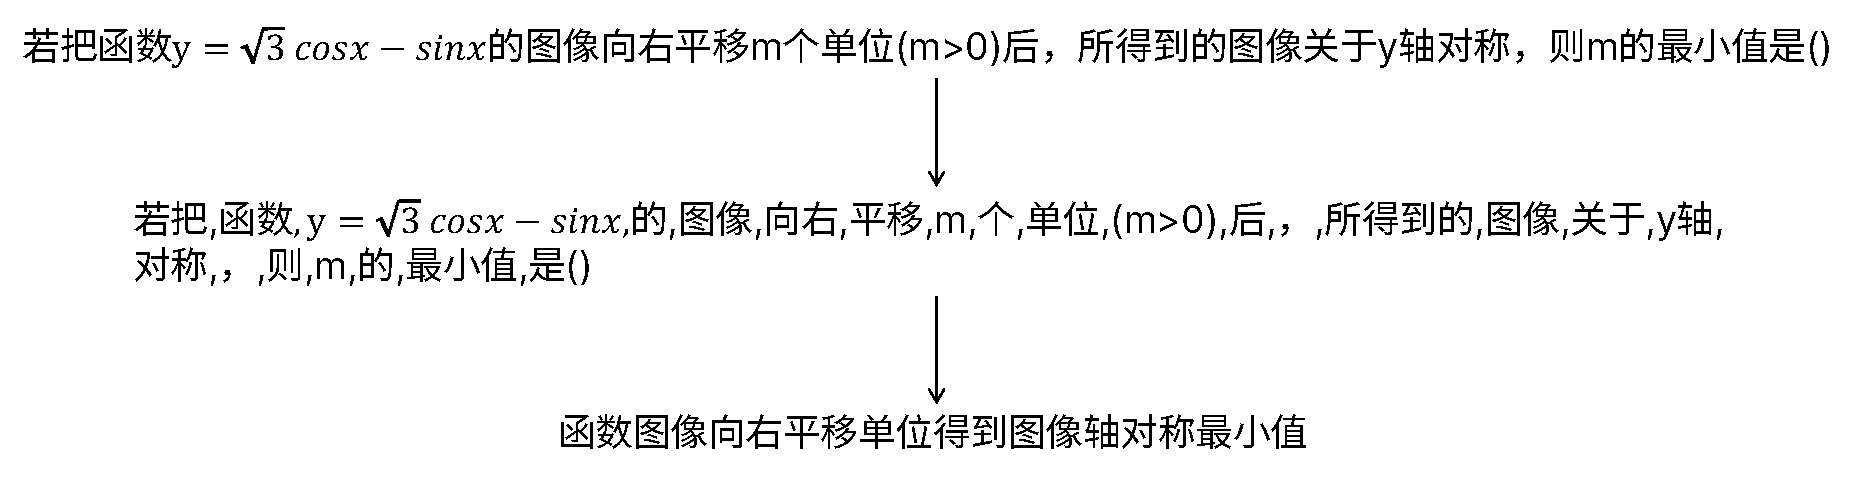
\includegraphics[width=1.0\textwidth]{ch2-model-preprocessing.pdf}
    \caption{Example of preprocessing}\label{fig:ch2-model-preprocessing}
\end{figure}

% - 分词。相对于其他表音语言如英语、西班牙语,中文语言预处理需要额外的分词步骤。在汉语中的词与词之间不存在自然分隔,因此需要人为对句子按照词义进行分割。选择合适的汉语分词算法可以为后续的处理奠定基础,提高整体模型性能。目前,汉语分词主要分为基于词典规则匹配和基于统计模型的两种算法。与前者相比,后者具有更好的泛化能力和学习能力。它用于先验规则之外的分词,如歧义词和未注册词表现较好。在该模型中,采用了目前流行的jieba分词,实现了基于Trie书结构的词条图扫描,利用阶段规划和HMM模型等算法,找到基于词频的最大分词分组和合并,实现了未来登录词的识别。用户还可以自定义停字和用户字典,实现专有名词识别。
% - 清理。语料库清理:保留语料库中的有用数据,删除噪声数据。常见的清洗方法包括:人工重删、对齐、删除和标注。对于句子中不需要的词,即停顿词,它们的存在不影响句子的意思。在文本中,会有大量的功能词、代词或没有特定含义的动词和名词。这些词对文本分析没有帮助,所以这些停顿词可以去掉。对于习题文本,有很多数学表达式、符号等,考虑到很多习题中的这些表达式不是文本格式,必须采用OCR技术将数学表达式从图片预处理成文本。因此,在中文文本足够的情况下,可以考虑将数学表达式过滤掉,以减少计算负荷。

\begin{itemize}
    \item Segmentation: Since original data has many ambiguous words and phrases, a word segmentation step is required to remove irrelevant words and phrases. In this step, the model removes irrelevant punctuation, stops words and words from the user dictionary. The user dictionary contains mainly redundant words from the text of mathematical exercises.
    \item Cleaning: Corpus cleaning preserves useful data in the corpus and deletes noisy data. Common cleaning methods include manual deduplication, alignment, deletion, and labeling. For words that are not necessary for a sentence, i.e., stop words, their existence does not affect the sentence's meaning. There will be many function words, pronouns, or verbs, and nouns with no specific meaning in the text. These words are not helpful to the text analysis so that these stop words can be removed. For the exercise description text, there are many mathematical expressions and symbols. Considering that these expressions in many exercises are not in text format, OCR technology must be applied to preprocess mathematical expressions from pictures to text. Therefore, when the Chinese text is sufficient, mathematical expressions can be removed to reduce the calculation load.
\end{itemize}

%经过数据处理的步骤,得到了一个干净的文本token序列,接下来在Embedding层可以利用BERT技术来进行文本embedding操作。
After the data processing step, a clean sequence of text tokens is obtained, and next in the Embedding layer, the BERT technique can be used to perform text embedding operations.

\subsubsection{BERT-Based Embedding Layer}
%在深度学习的应用过程中,嵌入是一种将符号形式的自然对象、模式等转化为数学空间中的向量的方法,是一种从离散空间到连续空间的转换,为神经网络在各方面的应用带来了极大的扩展。嵌入是一个将离散变量转为连续向量表示的一个方式。在神经网络中,embedding 是非常有用的,因为它不光可以减少离散变量的空间维数,同时还可以有意义的表示该变量。在词嵌入学习的研究中,有one-hot、Word2Vec和BERT等常见的词嵌入学习算法和模型。one-hot编码是最朴素的方法,它将所有的词语二进制化,即所有的词语只有存在或不存在两种情况,因此每个词语都是一个只有一个1其他全是0的二进制向量。当词语量较大时,该向量的长度也会相当长,在后续的计算也会产生大量的无效计算,即稀疏矩阵计算问题。Word2Vec由Google语2013年提出~\cite{church2017word2vec},它通过词语来预测它的上下文或者通过上下文来预测词语,是一种静态的词嵌入学习模式,但在解决多义词等问题上遇到瓶颈。Google于2018年提出的Bidirectional Encoder Representations from Transformers(BERT)模型利用Transformer作为基本单元,预训练masked语言模型,在几乎所有的自然语言处理任务都取得了State of the art(SOTA)的性能表现。它具有极强的语义表征效果。本文利用BERT来作为词Embedding向量学习模块,能更好地在不同习题文本的不同语境中取得更好的泛化和自适应能力。

In applying deep learning, embedding as a preprocessing approach for generating embedded vectors brings a great extension to neural networks' application in various aspects. In applying deep learning techniques, embedding is an instrumental skill because it reduces the spatial dimensionality of a discrete variable and allows a meaningful representation of that variable. For example, in NLP, if basic one-hot coding is used, it often results in invalid dimension and sparse vectors and also fails to learn the dependencies between vectors. The embedded vectors are updated during embedding training, which can clearly show the exercises between the vectors. The one-hot encoding is the most naive method, which turns all words into binary patterns, i.e., all words are only present or absent in two cases, so each word is a binary vector with only 1-value and all other 0-values. When the amount of words is large, this vector's length will also be quite long, and the subsequent computation will also generate a large number of invalid computations, i.e., the sparse matrix computation problem. Word2vec was proposed by Google Language 2013~\cite{church2017word2vec}, which predicts its context by words or predicts words by contexts, a static word embedding learning model, but encounters bottlenecks in solving problems such as polysemous words. The Bidirectional Encoder Representations from Transformers (BERT) model proposed by Google in 2018 utilizes the Transformer as the base unit to pre-train masked language models, achieving State of The Art (SOTA) performance in almost all NLP tasks. It has a powerful semantic representation effect. In this thesis, BERT is utilized as a word embedding vector learning module to achieve greater generalization and adaptive capabilities in different contexts of different idiomatic texts.

%在习题文本中,会出现一些组合词,即由多个词组合而成的具有不可分割词义的词组,由于在BERT的训练样本生成阶段,会对词进行mask操作,因此这些组合词有可能会被分别mask。导致出现歧义,引起训练性能退化。因此,本文应用全词mask的处理方式,该方法由cui等人于2019年提出~\cite{cui2019pre}。通过应用全词mask,当一个组合词的一个部分被mask,则该组合词的其他部分也会被mask。如图所示。


In the exercise description text, there will be some combinations of words, i.e., groups of words with indivisible lexical meanings formed by combining multiple words. Since the words are masked during the BERT training sample generation phase, these combinations may be masked separately, resulting in ambiguity and causing training performance degradation. Therefore, this thesis applies Whole Word Mask processing (WWM), proposed by Cui et al.\ in 2019~\cite{cui2019pre}. By applying WWM, when one part of a combined word is masked, then the other parts of that combined word are also masked, as shown in \figname{\ref{fig:ch2-bert-wwm}}.

\begin{figure}[htbp!]
    \centering
    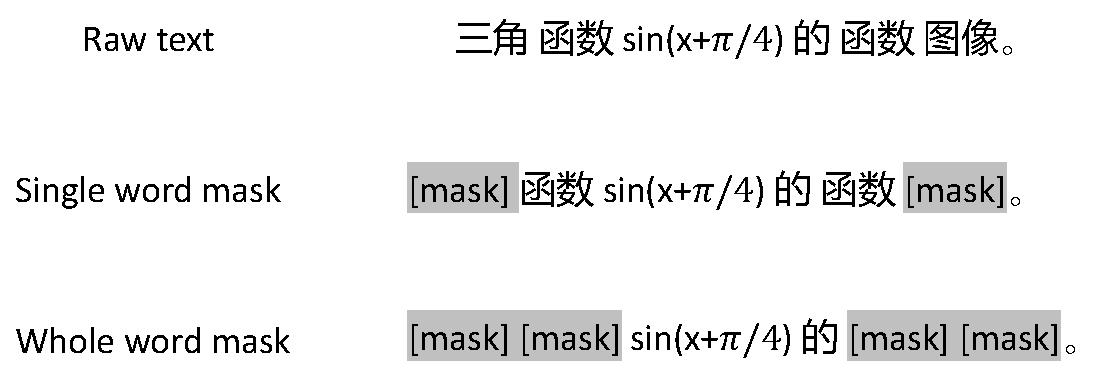
\includegraphics[width=0.8\textwidth]{ch2-bert-wwm.pdf}
    \caption{Whole word mask}\label{fig:ch2-bert-wwm}
\end{figure}

%将经过分词处理得到的习题文本词原始序列的部分词进行WWM处理,在序列的开头添加标记[CLS],句子间用[SEP]分隔符标示。经过训练,输出词embedding向量。每个词的输出embedding由三个部分组成,即token embedding、segment embedding和position embedding,它们从不同的角度对词进行嵌入信息表征。随后,将词嵌入向量输入BERT的特征提取双向Transformer层,可以获得包含深度语义特征的特征序列表征向量。整体架构如图所示。

WWM processes some words of the original sequence of exercise description text words obtained after the word separation process, and the marker [CLS] is added at the beginning of the sequence, and the inter-sentence is marked by [SEP] separator. After training, the word embedding vector is output. Each word's output embedding consists of three parts: token embedding, segment embedding, and position embedding, which characterize the word's embedding information from different perspectives. Subsequently, the word embedding vector is fed into the feature extraction bidirectional Transformer layer of BERT, and the feature sequence representation vector containing deep semantic features can be obtained. The overall architecture is shown in the \figname{\ref{fig:ch2-bert-model}}.

\begin{figure}[htb]
    \centering
    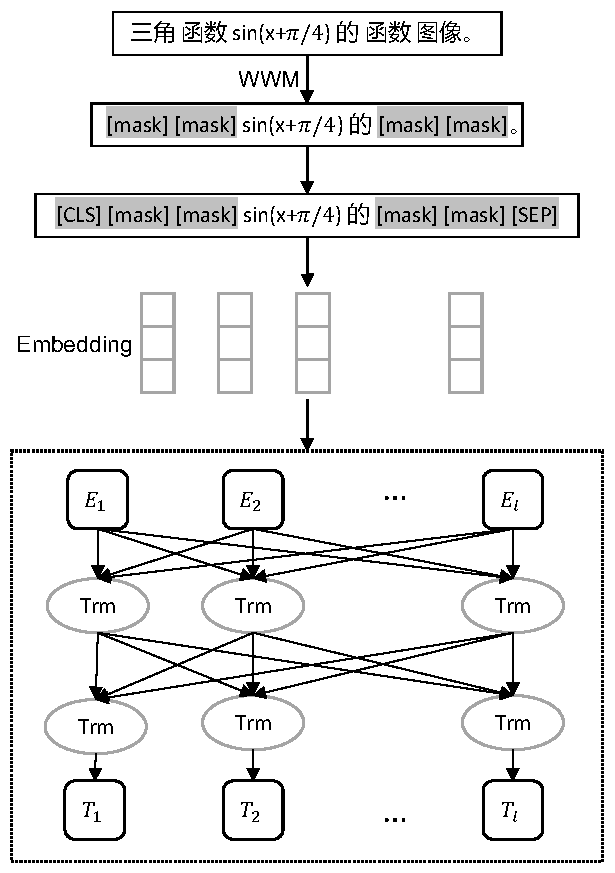
\includegraphics[width=0.7\textwidth]{ch2-bert-model.pdf}
    \caption{BERT-based embedding}\label{fig:ch2-bert-model}
\end{figure}

\subsubsection{Bidirectional LSTM Layer}
%在解决序列化模式数据建模方面,RNN具有良好的解决能力。在本节中,任务核心是一个序列到序列(Seq2Seq)的任务,输入一个题目描述的embedding向量,输出一个包含当前训练到的信息序列。最朴素的想法就是用原始的RNN,其结构如图所示,图中\(x_t\),\(h_t\)和\(y_t\)分别表示在时间t的输入值、隐藏值和输出值。

RNNs are well equipped to solve various types of problems and tasks in serialized pattern data modeling. In this section, the core of the task is a sequence-to-sequence (Seq2Seq) task, where an embedding vector described by the topic is input and a sequence containing the currently trained information is output. The most rudimentary idea is to use the original RNN.\@ Its structure is shown in the \figname{\ref{fig:ch2-rnn-model}}, where \(x_t\), \(h_t\) and \(y_t\) denote the input, hidden and output values at time \(t\), respectively. Then, the RNN training formula can be written as~\eqname{\ref{fml:rnn-train}}:

\begin{align}\label{fml:rnn-train}
    \begin{split}
        h^{t+1} & =f(W^h_{t} h^t+W^i x^t) \\
        y^{t+1} & =f(W^o h^{t+1})
    \end{split}
\end{align}


\begin{figure}[htbp!]
    \centering
    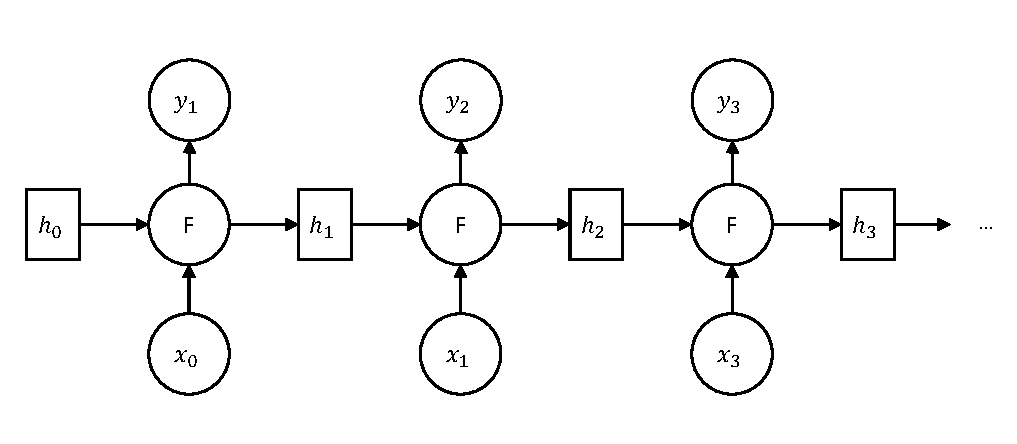
\includegraphics[width=1.0\textwidth]{ch2-rnn-model.pdf}
    \caption{Naive RNN unit}\label{fig:ch2-rnn-model}
\end{figure}

%但是,当序列较长时,就会出现长依赖性的问题。例如,对于一个序列,当前的状态依赖于离当前状态很远的一个状态,随着时间间隔的增加,RNNs学习这个状态的能力会大大降低。LSTM是作为针对RNN的这种缺陷的一种解决方案被提出来,它运用门控机制来实现长期记忆。解决RNN的梯度爆炸或梯度消失等问题。在捕捉序列信息方面也具有良好的性能。其结构如图所示,表示\(t\)时刻的一个LSTM单元内的计算细节。其中,\(\sigma\)为激活函数,\(c_t\)为单元状态表征,\(f_t\)为遗忘门控计算,\(i_t\)为输入门控计算,\(o_t\)为输出门控计算,\(h_t\)为隐藏状态表征。通过由门控控制的遗忘机制,可以有效建模对于远距离序列单元信息。

However, when the sequence is long, the problem of long dependencies arises. For example, for a sequence, the current state depends on a state far away from the current state, and as the time interval increases, the ability of RNNs to learn state representation is greatly reduced. Long short-term memory (LSTM)~\cite{lstm1997, lindemann2020survey}, as a solution to overcome shortcomings of RNN, which uses a gating mechanism to achieve long-term memory. It solves the problems such as gradient explosion or gradient disappearance of RNN. It also has a good performance in capturing sequence information. The general model of LSTM is like \figname{\ref{fig:ch2-lstm-model}}, which represents the computational details within an LSTM cell at the moment of \(t\). Among them, \(\sigma\) is the activation function, \(c_t\) is the cell state representation, \(f_t\) is the forgetting gating calculation, \(i_t\) is the input gating calculation, \(o_t\) is the output gating calculation, and \(h_t\) is the hidden state representation. The forgetting mechanism controlled by gating can be effectively modeled for long-range sequential unitary information.

\begin{figure}[htbp!]
    \centering
    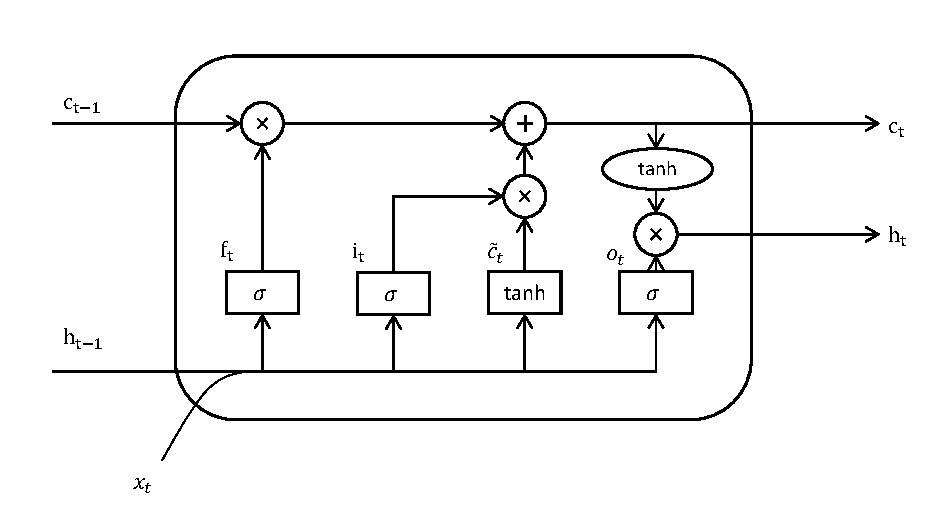
\includegraphics[width=1.0\textwidth]{ch2-lstm-model.pdf}
    %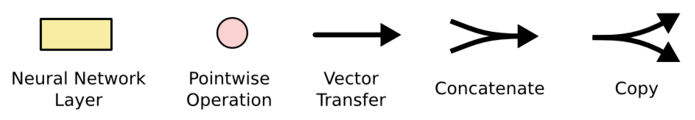
\includegraphics[width=1.0\textwidth]{ch2-fig8.png}
    \caption{Structure of LSTM unit}\label{fig:ch2-lstm-model}
\end{figure}

%单向LSTM也有一个固有的缺陷,它只能捕获\(t\)时刻以前的序列状态信息,即只能捕获之前序列输入。双向LSTM通过将反向序列输入LSTM并与正向LSTM序列进行聚合,可以捕获双向的语义信息,同时对双向的依赖建模。
One-way LSTM also has an inherent drawback that it can only capture the sequence state information before \(t\) moment, i.e., it can only capture the previous sequence input. The bidirectional LSTM (Bi-LSTM) can capture semantic information in both directions by feeding the reverse sequence into the LSTM and aggregating it with the forward LSTM sequence while modeling the dependencies in both directions~\cite{liu2019bidirectional}. The Bi-LSTM output can be obtained by inputting the positive sequence and the reverse sequence input sequence into two sets of LSTM networks and perform element-wise addition. The output of positive-order LSTM is \(\overrightarrow{h_t}\), the output of reverse-order LSTM is \(\overleftarrow{h_t}\), \(\bigoplus \) means sequence concatenation. The output of Bi-LSTM is shown in \figname{\ref{fml:ch2-bilstm-output}}.
\begin{align}\label{fml:ch2-bilstm-output}
    \begin{split}
        \overrightarrow{h_t} & = \overrightarrow{LSTM}(e_t)                       \\
        \overleftarrow{h_t}  & = \overleftarrow{LSTM}(e_t)                        \\
        h_t                  & =\overrightarrow{h_t}\bigoplus \overleftarrow{h_t}
    \end{split}
\end{align}
The Bi-LSTM Structure is like \figname{\ref{fig:ch2-model-bilstm}}.

\begin{figure}[htb]
    \centering
    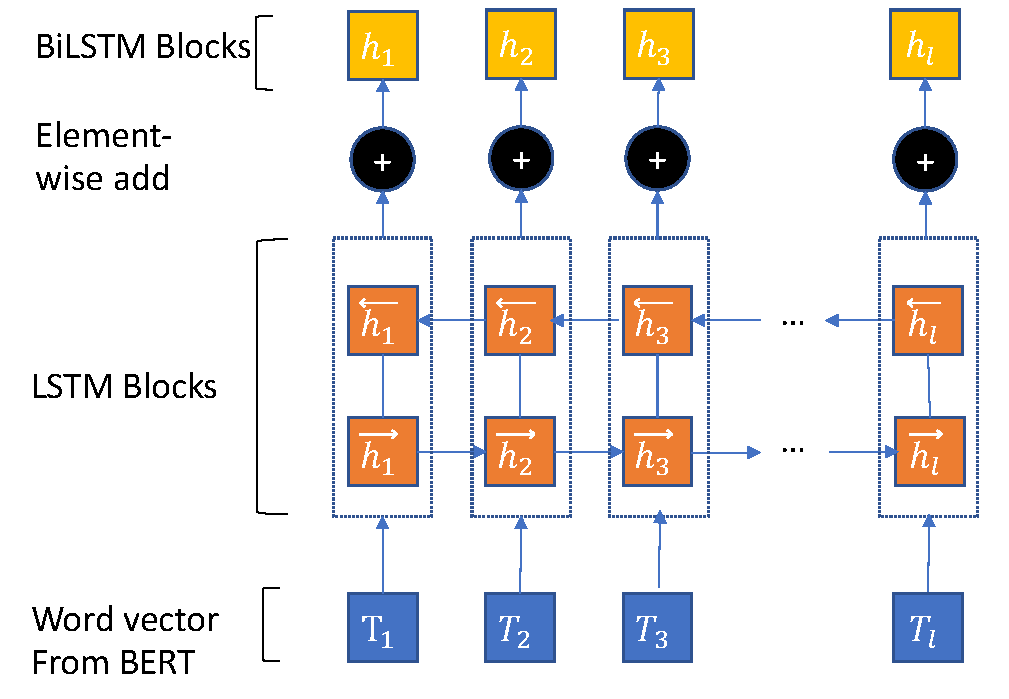
\includegraphics[width=.9\textwidth]{ch2-bilstm-model.pdf}
    \caption{Structure of Bi-LSTM}\label{fig:ch2-model-bilstm}
\end{figure}

Here, the Bi-LSTM output a bidirectional sequence as the concatenation of positive-order and reverse-order LSTM output sequence. It is a higher-order representation of the exercise text's sentence vector, and the model can also be stackable with multiple Bi-LSTM layers to characterize the deep sentence sense vector~\cite{jang2020bi}.



\subsubsection{Attention Layer}

%由于文本挖掘任务中,每个特征词对于总体语义的影响是非对称的,即关键词在决定整个文本的含义方面有决定性的作用。Bahdanau等人提出的~\cite{bahdanau2014neural}提出了Attention机制模型正是基于这一原理。人的注意力是一种聚焦于关键信息忽略非关键信息的机制,即各个信息点的权重不一样。

%按照注意方法,编码器使用Bi-LSTM并获得隐藏状态向量 \(h_t = \ overrightarrow {h_t}) \ bigoplus \ overleftarrow {h_t} \)。在解码器阶段,计算每个编码器隐藏层状态和解码器隐藏层状态之间的相关性,并执行softmax归一化操作以获得每个隐藏层矢量的权重。将\(H\)设置为\(H = [h_1,h_2,...,h_l] \)  的隐藏状态矩阵,我们可以计算嵌入\(r\)的练习文本。计算公式如下:


Since each feature word's impact on the overall semantics in a text mining task is asymmetric, i.e. keywords have a decisive role in determining the meaning of the entire text~\cite{chaudhari2020attentive}. Human attention is a mechanism that focuses on key information ignoring non-key information, i.e., individual information points are weighted differently. This method achieved remarkable results in different tasks such as image vision~\cite{fu2017look,sun2018multi}, language mining~\cite{hu2019introductory}, and voice recognition~\cite{chorowski2015attention} and is applied widely.


Human attention is a mechanism for quickly screening high-value information from massive information. The human attention mechanism inspires the deep learning attention mechanism. This method is widely used in various types of deep learning tasks such as NLP~\cite{hu2019introductory}, image classification~\cite{fu2017look,sun2018multi}, and speech recognition~\cite{chorowski2015attention}, and has achieved remarkable results.

\begin{figure}[htb]
    \centering
    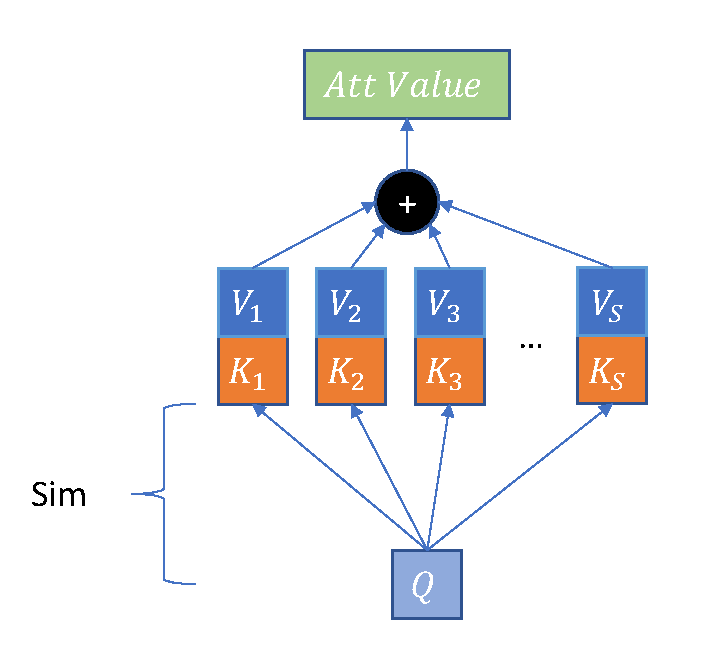
\includegraphics[width=0.7\textwidth]{ch2-model-attmodel.pdf}
    \caption{The essential idea of attention mechanism}\label{fig:ch2-model-attmodel}
\end{figure}


The essence of the attention mechanism is a group of key-value pairs \(<K, V>\) contained in Source \(S\), given an element of Query \(Q\), which is followed by calculating the \(Q\) similarity to each \(K\) and remembering the weight coefficients of the corresponding values \(V\). It is showed in \figname{\ref{fig:ch2-model-attmodel}}. Then a weighted sum is performed to obtain the final Attention value. It can be expressed as \eqname{\ref{fml:ch2-attention}}, where \(Att\) and \(Sim\) represent attention and similarity.
\begin{align}\label{fml:ch2-attention}
    Att(Q,S) = \sum_{i=1}^{|S|}Sim(Q,K_i)*V_i
\end{align}

%本节的注意力机制的核心原理是计算出对句义影响最大的词,即关键语义词,它们在之后被汇总成为句义表征向量。
Following the attention method, the encoder use Bi-LSTM and get hidden state vector \(h_t=\overrightarrow{h_t}\bigoplus \overleftarrow{h_t}\). A word attention mechanism is introduced here. The core principle of the attention mechanism in this section is to compute the words that have the greatest influence on sentence meaning, i.e., the key semantic words, which are later aggregated into a vector of sentence meaning representations. The formula is \eqname{\ref{fml:ch2-att2}}, where \(u_t\) is the hidden representation of \(h_t\), \(r\) is the output text vector, and the \(u_\omega \) is the similarity of the text vector of word aspect. By measuring the similarity between \(u_t\) and \(u_\omega \) as the importance of the word, and using the softmax function to calculate normalization and to obtain the importance weight \(\alpha_{t}\). Finally, the entire text is transformed to word representation based on semantic contribution weights.

%
After that, the entire text is represented as a weighted sum of word vectors. The context vector \(u_\omega \) can be regarded as a high-level representation of the fixed query ``what is the word conveying information'' and is randomly initialized as a learnable parameter in training.


\begin{align}\label{fml:ch2-att2}
    \begin{split}
        u_t      & = \tanh(W_\omega h_t + b_\omega )                                                    \\
        \alpha_t & =Softmax(u_t^T u_\omega) = \frac{\exp( u_t^T u_\omega)}{\sum_t \exp(u_t^T u_\omega)} \\
        r        & = \sum_t{\alpha_t h_t}
    \end{split}
\end{align}

\subsection{The GCN-based Knowledge Point Classifier Generator}
%在高中数学学科中,知识点之间具有较为复杂的相互关联例如相关、从属、包含、前驱、后继等等。这些复杂的相互关系在欧式空间往往难以建模,或这产生数据稀疏性的问题。而通过图数据结构来建立知识点间的关系则更加直观和拥有更好的解释性。回顾本模型的任务,它给出习题的描述、答案,部分已经标记好知识点,利用这些信息来对为标注知识点的习题进行知识点标注。考虑到知识点之间的依赖关系,一些在浅层特征上无法表征的深层隐藏知识点也可以通过图神经网络输出分类器被正确标注。在本模型中,用到了图卷积神经网络来建模知识点关系图,每个知识点都对应图上的一个节点。经过多个图卷积计算,生成一系列的分类器,这些分类器分别作用在文本挖掘模块产生的文本向量,每个分类器输出一个值表征该知识点与是该习题相关联的概率。其总体架构如图所示。

%本模型采用GCN结构的原因在于,GCN对于各个节点的参数共享使得学习到的分类器可以保留知识关联图中的关联信息,从而隐式表示其空间语义结构。因此输出的分类器可以保留和识别隐式知识标签依赖信息。 对于知识点的依赖关系参考数据关联方法挖掘算法例如apriori算法,通过计算知识点在习题中的共现度来计算其协关系矩阵。

In high school mathematics, knowledge points have more complex interrelationships such as correlation, subordination, inclusion, predecessor, successor, etc. These complex interrelationships are often difficult to model in Euclidean space, or this creates data sparsity problems. The establishment of relationships between knowledge points through graph data structures is more intuitive and has better interpretability. Recalling this model's task, it gives descriptions and answers to exercises, some of which have already marked knowledge points, and uses this information to mark knowledge points for exercises that are labeled knowledge points. Considering the dependence between knowledge points, some deeply hidden knowledge points that cannot be represented in shallow features can also be correctly labeled by the graph neural network output classifier. In this model, a GCN is used to learn and form the knowledge point connection graph, and each knowledge point corresponds to a node on the graph. After multiple graph convolution calculations, a series of classifiers are generated. These classifiers respectively act on the text vector generated by the text mining module. Each classifier outputs a value representing the probability that the knowledge point is associated with the exercise. Its overall structure is shown in the \figname{\ref{fig:ch2-gcn-ov}}.

\begin{figure}[htbp!]
    \centering
    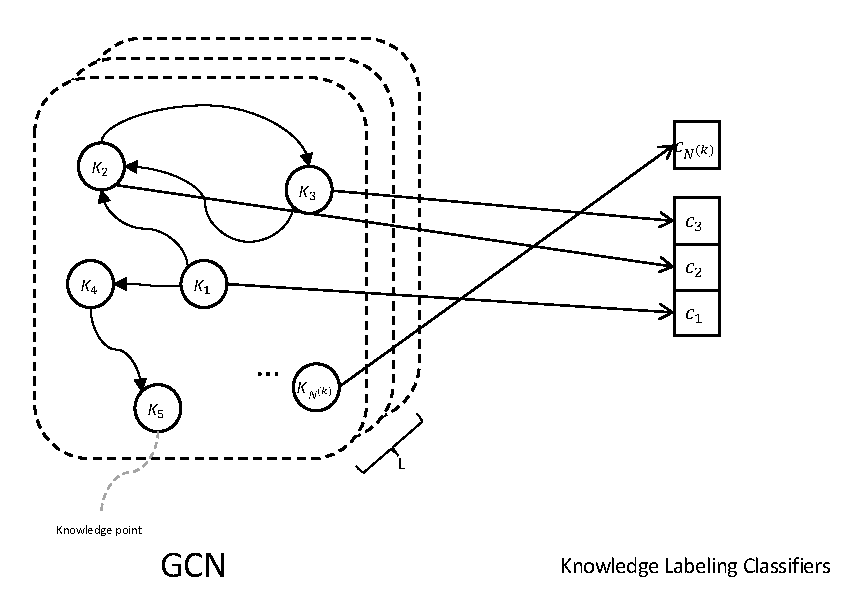
\includegraphics[width=0.8\textwidth]{ch2-gcn-ov.pdf}
    \caption{The overview of structure}\label{fig:ch2-gcn-ov}
\end{figure}



\subsubsection{Graph Convolutinal Network}
%在现实世界中,许多重要的数据集都以网络的形式产生连接,形成图状结构。一些论文对此问题进行了回顾,并试图对神经网络进行概括,并将其应用于任意图结构数据~\cite{wu2018socialgcn,dettmers2018convolutional}。图卷积神经网络(GCN)~\cite{kipf2016semi}用于处理传统卷积神经网络难以学习的非欧氏空间数据。它定义在一个图结构\(G=(V,E)\)上,其中\(V\)、\(E\)为图的顶点和边。GCN的输入为维度为\(n^v\times d^{v}\),其中\(n^v\)为节点数,\(d^v\)为各个顶点的特征维度数。此外,GCN又一个用于描述图结构的维度为\(n^v\times n^v\)的邻接矩阵\(A\)。

In the real world, many important data sets generate connections as networks that form graph-like structures. Some researchers reviewed this problem and attempted to generalize neural networks and apply them to arbitrary graph-structured data~\cite{wu2018socialgcn, dettmers2018convolutional}. The GCN~\cite{kipf2017semi} is used to process non-Euclidean spatial data that are difficult to learn by traditional convolutional neural networks. It is defined on a graph structure \(G=(V, E)\), where \(V\) is the denote of vertex and \(E\) is the denote of edge inside the graph. The input of GCN \(X = H^{(0)}\) is the first layer of GCN. The ith layer is denoted as \(H^{(i)}\), and \(H^{(i)}\in \mathbb{R}^{N^{(v)}\times d_{i}}\), where \(N^{(v)}\) is the denote of number of vertexes and \(d_{i}\) is the number of dimension of each vertex of layer \(i\). The output layer \(Z = H^{(L)}\) where L is the number of layers in GCN\@. Also, the GCN has another adjacency matrix \(A\) of dimension \(N^{(v)}\times N^{(v)}\) used to describe the graph structure.

%图卷积的学习的核心是传播,即每个节点都会传播信息给邻接的节点。每一层的传播都会被聚合起来形成下一层。GCN的第\(i-1\)层\(H^{i-1}\)到第\(i\)层\(H^i\)转换可以写作公式\ref{fml:ch2-gcnlayer},其中f为特定的传播方式,例如所有的节点将自身的值均匀扩散给邻接节点。
The core of graph convolutional learning is propagation, i.e., each node propagates information to neighboring nodes. The propagation of each layer is aggregated to form the next layer. The \(i-1\) layer \(H^{(i)}\in \mathbb{R}^{N^{(v)}\times d_v}\) to layer \(H^{(i+1)}\) transformation of GCN can be written in the formula \eqname{\ref{fml:ch2-gcnlayer}}, where \(f(\cdot)\) is a specific propagation method, e.g.\ all nodes spread their own values uniformly to neighboring nodes.

\begin{align}
    \begin{split}
        H^{(i+1)}=f(H^{(i)},A) \label{fml:ch2-gcnlayer}
    \end{split}
\end{align}

%知识点间关系可以通过相关矩阵来表示,即当知识点\(i\)与知识点\(j\)相关,相关矩阵为了学习知识点之间的表示,将知识点建模为GCN中的一个顶点。该关系通过共现概率来进行学习,即对经过标记知识点的习题库进行监督学习。这是基于如下假设:当多个知识点在一个习题中出现概率较大,则其应当存在内在联系。

A correlation matrix can represent the relationship between knowledge points, i.e., when a knowledge point \(i\) is related to a knowledge point \(j\), the correlation matrix \(A\) models the knowledge point as a vertex in the GCN in order to learn the representation between knowledge points. The relation is learned by co-occurrence probability, i.e., supervised learning is performed on the library of exercises that have been tagged with knowledge points, which is based on the assumption that when multiple knowledge points have a high probability of occurring in an exercise, they should be intrinsically linked.

%本节中GCN的节点传播方式为\ref{fml:ch2-gcn2},其中\(\tilde{A}\)为\(A\in \mathbb{R}^{N^{(v)}\times N^{(v)}}\)的正则化。\(h\)为非线性激活函数,这里选用LeakyReLU~\cite{maas2013rectifier}。需要学习的参数矩阵\(W^{(i)}\in \mathbb{R}^{d_{i}\times d_{i+1}}\)可以通过习题知识点的统计关系来计算。

The node propagation of GCN in this section is~\eqname{\ref{fml:ch2-gcn2}}, where \(\widehat{A}\) is the normalization form of \(A\in \mathbb{R}^{N^{(v)}\times N^{(v)}}\). The \(h(\cdot)\) is the nonlinear activation function LeakyReLU~\cite{maas2013rectifier}. The parameter matrix \(W^{(i)}\in \mathbb{R}^{d_{i}\times d_{i+1}}\) to be learned can be calculated by the statistical relations of the exercise knowledge points. The training process of Proposed is shown in \figname{\ref{fig:ch2-gcn-explain}}.
\begin{align}
    \begin{split}
        H^{(i+1)} = f(\tilde{A}H^{(i)}W^{(i)})\label{fml:ch2-gcn2}
    \end{split}
\end{align}

\begin{figure}[htbp!]
    \centering
    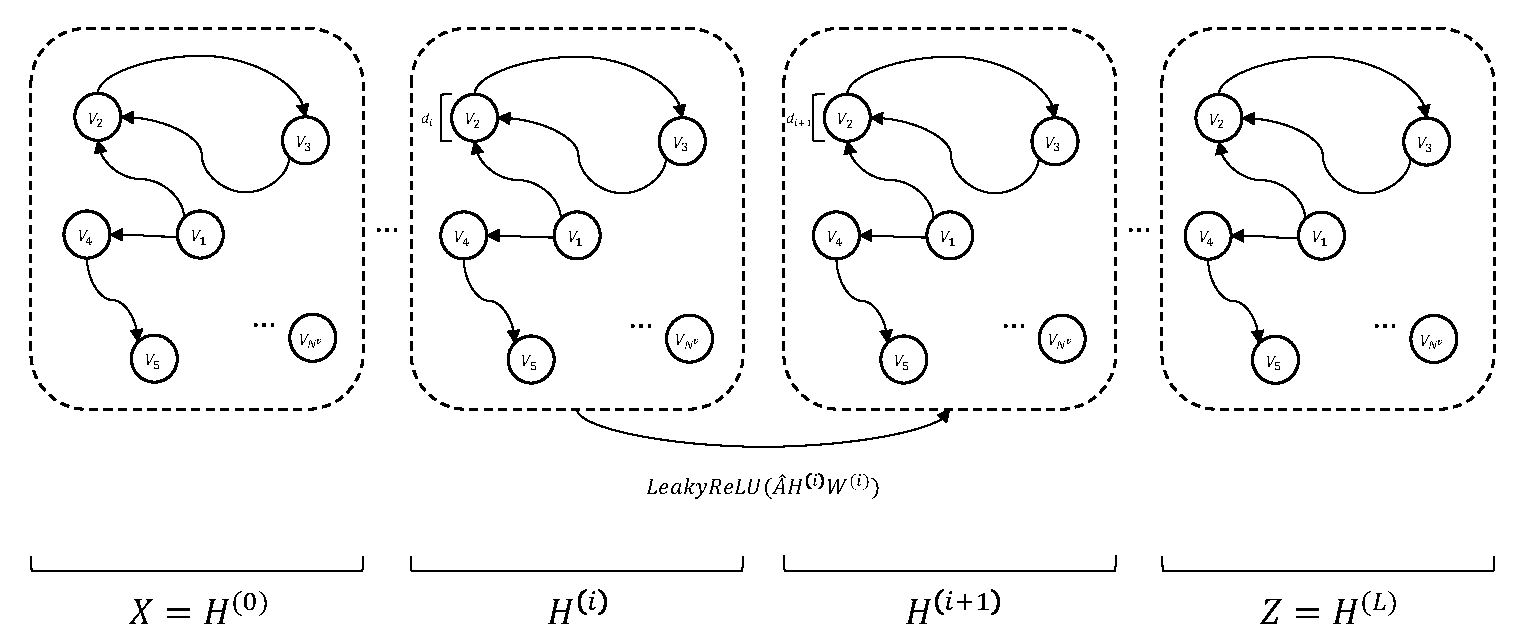
\includegraphics[width=1.0\linewidth]{ch2-gcn-modelov.pdf}
    \caption{The GCN training process}\label{fig:ch2-gcn-explain}
\end{figure}

%在本模型中,每个节点都是知识点的表征,在此可以通过知识点文本表征向量来进行表征。通过对相关知识点的图传播学习,可以使相关知识点的表征产生融合,进而提升模型识别对于相关知识点的联想学习性能。
In this model, each node represents a knowledge point. The graph input is the word embedding of the label. As the model integrates the text information of labels, so each node has latent relation with exercises represented with a text representation vector, which is the underlying principle of this model. The graph propagation learning of related knowledge points can produce the fusion of related knowledge point representations, which improves the associative learning performance of model recognition for related knowledge points.

\subsubsection{Design of Correlation Matrix}
%在GCN中,相关矩阵\(A\)表征了图节点之间的关系,GCN信息传播计算也是基于\(A\)进行的。因此,设计相关矩阵\(A\)是GCN模型的关键步骤。在该模型中,采用常用的数据关联规则挖掘算法Apriori算法,通过知识点共现次数统计来计算关联。 

%在该模型中,其实只需要找到知识点的对偶关系。因此,知识点关系矩阵可以表示为\(R/in \mathbb{R}^{T\time T}\)。第一个任务是找到标签集中频繁关联标签的出现次数。\(\operatorname{Support}\)、\(\operatorname{Confidence}\)和\(\operatorname{Lift}\)可以用来评估频繁标签集。支持度是指标签集中标签对的出现次数占总标签集的比例。置信度反映了一个标签\(L_i\)出现、另一个标签\(L_j\)出现的概率,或数据的条件概率。提升度表示标签\(L_i\)$同时包含的概率,以及X种群出现概率的比例。

In GCN, the correlation matrix \(A\) characterizes the relationship between graph nodes, and GCN information propagation calculation is also based on \(A\). Therefore, designing the correlation matrix \(A\) is a crucial step in the GCN model. In this model, the commonly used data association rule mining algorithm Apriori algorithm calculates knowledge point association by knowledge point reference co-occurrence statistics.

In this model, only the knowledge pairwise relationship needs to be found. Therefore, the knowledge point relationship matrix can be expressed as \(R\in \mathbb{R}^{T\times T}\). The first task is to find the number of occurrences of frequently associated label in the label set. The \(\operatorname{Support}\), \(\operatorname{Confidence}\), and \(\operatorname{Lift}\) can be used to evaluate frequent label sets. Support is the proportion of the number of occurrences of label pair in the label set in the total label set. Confidence degree reflects the probability of a label \(L_i\) appearing, another label \(L_j\) appears, or the conditional probability of the data. Lift represents the probability that the label \(L_i\) is contained at the same time, and the ratio of the probability of occurrence of X population:
\begin{align}
    \begin{split}
        \operatorname{Support}(L_i, L_j)       & =P(L_i,L_j)=\frac{\operatorname{number}(L_i,L_j)}{\operatorname{number}(\text{ All Samples })} \\
        \operatorname{Confidence}(L_i \to L_j) & =P(L_i \mid L_j)=P(L_i, L_j) / P(L_j)                                                \\
        \operatorname{Lift}(L_i \to L_j)       & =P(L_i \mid L_j) / P(L_i)=\operatorname{Confidence}(L_i \to L_j) / P(L_i)
    \end{split}
\end{align}

Similar to calculating Support, the frequency matrix \(E\in \mathbb{R}^{N^{(k)}\times N^{(k)}}\) of the sample knowledge point label pairs in the exercise training set can be calculated here. The \(M_{ij}\) represents the amount of co-occurrence between the knowledge point \(i\) and the knowledge point \(j\) in an exercise reference. Similarly, the knowledge point pair can be calculated by calculating Confidence to calculate the conditional probability matrix \(P\), where \(P_{ij}=P(L_i, L_j)/P(L_j)\), where \(P_{ij}=P(L_i, L_j)/P(L_j)\) means the situation when the knowledge point \(j\) appears The conditional probability of the occurrence of the following knowledge point \(i\).

It is a simple solution to directly set \(P\) as the incidence matrix \(A\), but in actual situations, some comprehensive questions in the exercise set contain practically unrelated knowledge points, but these situations are relatively rare. In order to exclude the interference of accidental circumstances, a minimum knowledge confidence threshold can be set. When \(P_{ij}\) is greater than the given threshold \(\tau^{(k)} \), naming activating value, then \(A_{ij}\) is set to \(P_{ij}\), Otherwise \(A_{ij}\) is set to 0. The formula is like \eqname{\ref{fml:confidence}}.

\begin{align}
    A_{ij}=\{\begin{array}{ll}
        0,      & \text{ if } P_{ij}<\tau^{(k)}      \\
        P_{ij}, & \text{ if } P_{ij} \geq \tau^{(k)}
    \end{array}\label{fml:confidence}
\end{align}


%该模型之所以采用GCN结构,是因为GCN对每个节点的参数共享,使得学习到的分类器可以在知识关联图中保留相关信息,从而隐性地表达其空间语义结构。因此,输出的分类器可以保留和识别隐含的知识标签依赖信息。对于知识点的依赖性,可以参考数据关联法挖掘算法,如apriori算法,通过计算习题中知识点的共现性来计算共相关矩阵。

This model adopts the GCN structure because the parameter sharing of GCN for each node allows the learned classifier to retain the associated information in the knowledge association graph, thereby implicitly expressing its spatial semantic structure. Therefore, the output classifier can retain and identify the implicit knowledge label dependent information. For the dependence of knowledge points, refer to the data association method mining algorithm such as Apriori algorithm~\cite{panjaitan2019implementation}, and calculate the correlation matrix by calculating the co-occurrence of knowledge points in the exercises.


\subsubsection{Classifier generator}

%在所提出的基于GCN的模型中,知识点标签用词嵌入来表示。知识点集 \(K={k_1,k_2,\ldots,k_T} \),其中 \(T\)为知识点的总数。对于每一个单个知识点来说\(k_i\),\(k_i \in mathbb{R}^{Ttimes d^{(k)}}),\(d^{(k)})是知识点对象的嵌入向量的维度。本文采用可学习的堆栈式GCN网络将这些知识点对象逐一转化为内部连接的知识点对象分类器\(C=[c_1,c_2,\ldots,c_n]\),其中\(c_iin\mathbb {R}^{Ttimes d^{(r)}}\),\(d^{(r)}\)是文本挖掘模块输出的文本表示向量\(r\)的维度。这些分类器和\(r\)可以用来计算每个标签的点积。

In this thesis, a learnable stacked GCN-based model for knowledge relation representation is proposed. The knowledge point labels are represented by knowledge label word embedding. Knowledge point set \(K=\{k_1,k_2,\ldots,k_{N^{(k)}}\} \), where \(N^{(k)}\) denotes the amount of knowledge points. For each single knowledge point \(k_i\), it is constrained that \(k_i \in \mathbb{R}^ {d^{(k)}}\), in which \(d^{(k)}\) is the dimensionality of the embedding vector of knowledge point object. The knowledge label word embedding set is the input of GCN, i.e., \(X = K\). The GCN is used to transform these knowledge point objects one by one into an internally connected knowledge point object classifier \(C=[c_1,c_2,\ldots,c_{N^{(k)}}\), where \(c_i \in \mathbb {R}^{d^{(r)}}\), \(d^{(r)}\) is the dimensionality of the text representation vector \(r\) output by the text mining module. These classifiers and \(r\) can be used to calculate the dot product of each label. The structure overview is proposed in \figname{\ref{fig:ch2-gcn-clsgen}}.

\begin{figure}[htbp!]
    \centering
    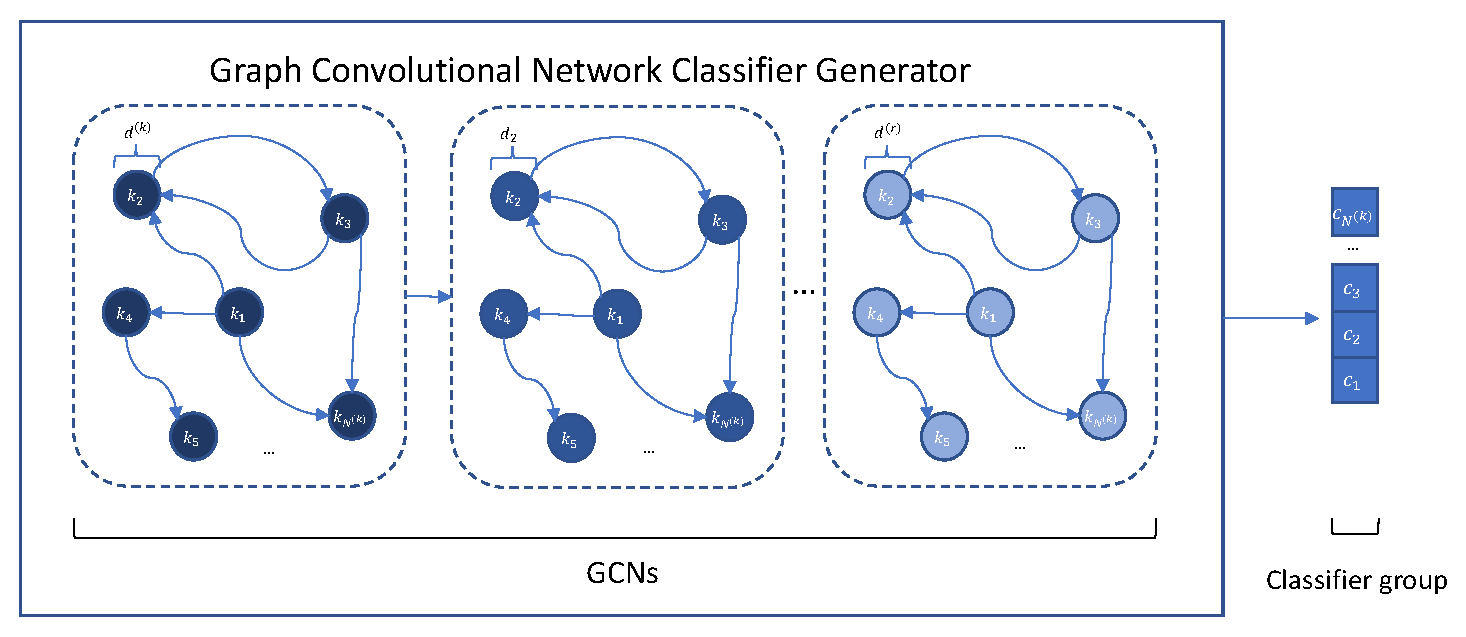
\includegraphics[width=1.0\linewidth]{ch2-gcn-clsgen.pdf}
    \caption{The structure of GCN-based classifier generator}\label{fig:ch2-gcn-clsgen}
\end{figure}

\subsection{Multi-label Recognition}
%  For the input layer, the input is \(r\in \mathbb{R}^{T \times d^{(k)}}\), where \(d^{(k)}\) is the number of dimensions represented by the embedding of the knowledge point object. Each GCN layer 1 takes the node representation from the previous layer \(H^{(l)}\) as input and outputs a new node representation \(H^{(l+1)}\). The output layer of the last layer is \(C\), where \(d_r\) represents the dimension of the title text. 

From the stacked GCN network, the object classifiers \(C=\{c_1,c_2,\ldots,c_{N^{(k)}}\} \) can be learned, where \(N^{(k)}\) represents the number of knowledge points. Finally, the label prediction vector \(\hat{y}\) can be obtained by the dot product of the learned classifier and the title text representation \(r\) as shown in \eqname{\ref{fml:ch2-classifier-mul}}.
\begin{align}\label{fml:ch2-classifier-mul}
    \hat{y} = C\times r
\end{align}

Through manual labeling, the real knowledge point labels of the exercises can be obtained: \(y\in \mathbb{R}^C\), \(y_i\in \{0,1\} \), \(y_i=0\) means that the exercise does not have knowledge points The label of \(i\), on the contrary, \(y_i=1\) means that the exercise has a label of knowledge point \(i\). The loss function \(\mathbf{L}\) can be written as~\eqname{\ref{fml:ch2-lossfunction}}.
\begin{align}\label{fml:ch2-lossfunction}
    \mathbf{L}=\sum_{i=1}^{T} y_i \log (\text{sigmoid}(\hat{y}_i))+(1-y_i) \log (1-\text{sigmoid}(\hat{y}_i))
\end{align}

\section{Experiments}
%本章提出了一个习题知识点多标签标注的模型,在本节中,先对数据集进行了介绍,接着介绍了一些Baseline性能的模型,然后结合多标签标注提出了对比的性能指标评估方案,最后给出对比结果和分析。This chapter proposes a multi-label labeling model for exercise knowledge points. 
This section first introduces, preprocess, and analysis the dataset, then introduces some baseline performance models, followed by the introduction of multi-label labeling metrics. Finally, comparison results and analysis are given.
\subsection{Dataset}
%本文中的实验数据来自于在线网站tiku.21cnjy.com的带标签的高考数学考题以及模拟题(包含答案解析),通过爬虫爬取题干、答案解析等文本语料。其部分知识点关联模型可以表示为如下图结构。该数据集经过过滤和人工选择,共3374道试题,包含148个知识点,题均知识点为1.7个,其知识点分布如图所示。
The experimental data are the labeled math examination questions and practicing exercises (including answer analysis) fetched from the online exercise website ``tiku.21cnjy.com''. The text corpus, such as exercise texts and answer analysis, are crawled through web crawlers. The raw data are roughly classified text records that contain a lot of repetitive redundancy and error information, so a data preprocessing process is needed to filter out the appropriate data. The knowledge graph of the original dataset is shown in the \figname{\ref{fig:ch2-model-knowledgenet}}.
\begin{figure}[htbp!]
    \centering
    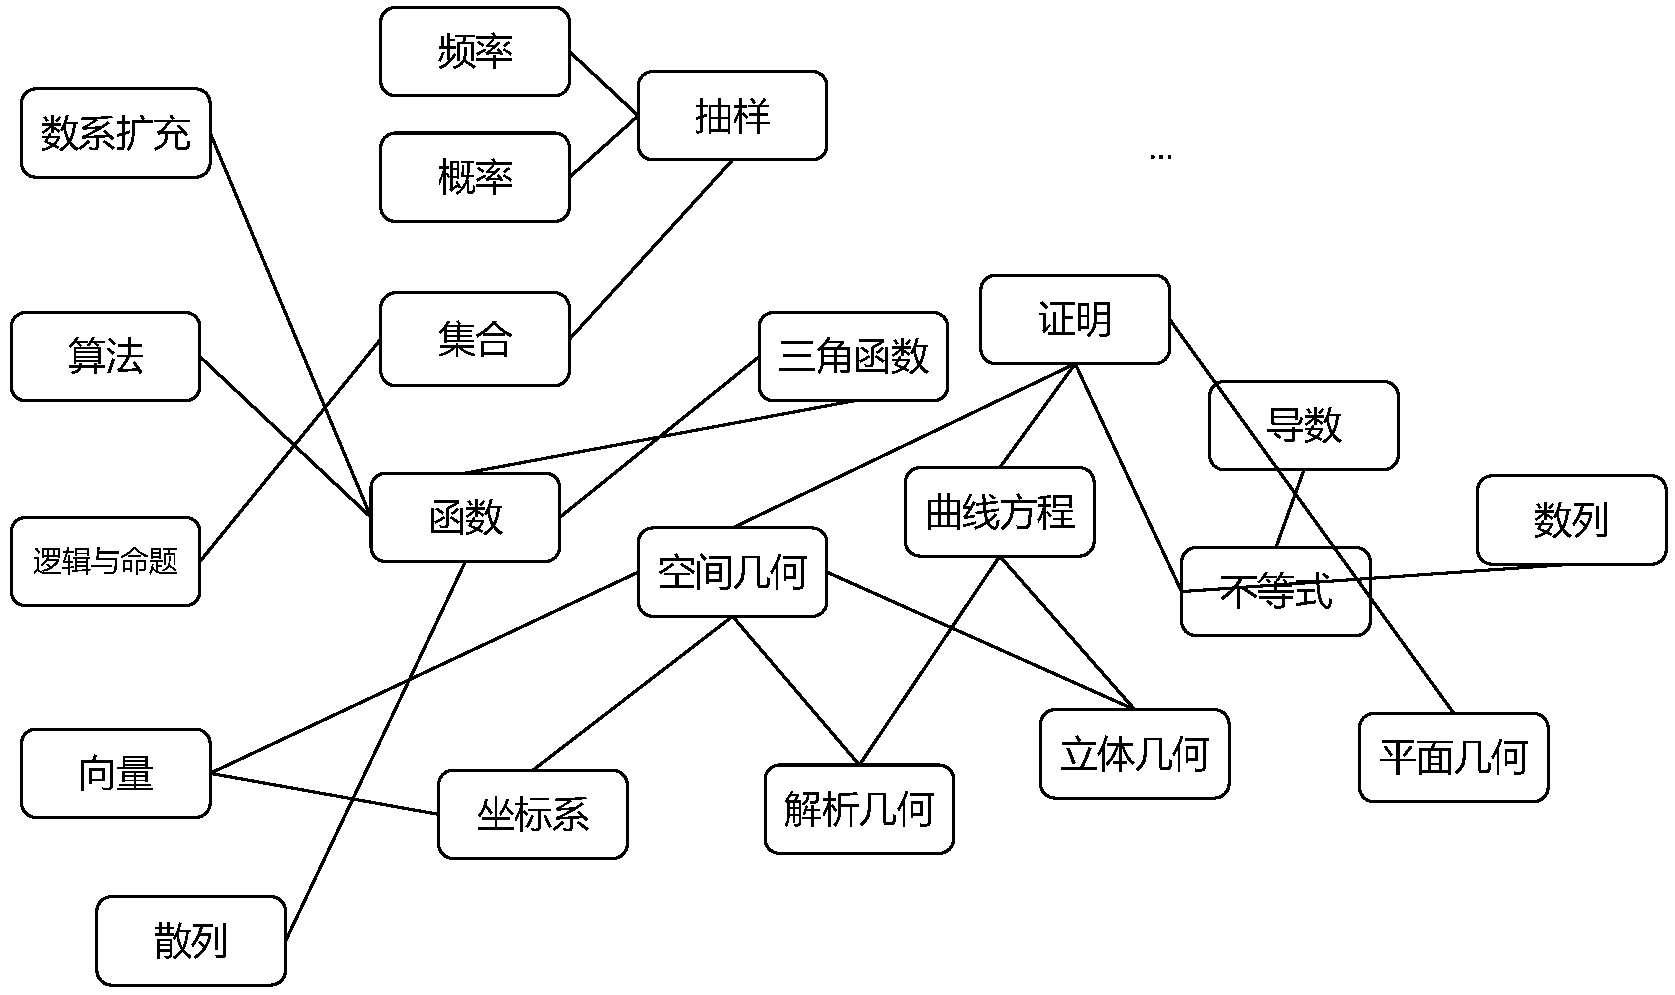
\includegraphics[width=1.0\textwidth]{ch2-model-knowledgenet.pdf}
    \caption{Knowledge point relation graph of original dataset}\label{fig:ch2-model-knowledgenet}
\end{figure}

\subsubsection{Data Preprocess}
This section uses web crawlers to obtain the data, so the original data obtained contains many unstructured exercises with irregular mathematical symbols, which will bring errors so that the unrecognizable characters will be replaced in the preprocessing process. There is also a large amount of nonsensical text. Besides, since some of the exercises are not fully labeled with knowledge points, manual assistance is required to label the dataset's training knowledge points.


\subsubsection{Data Analysis}
Since there are many images in the original set of exercises that cannot be identified, this question screens out irrelevant image URL information. This model does not consider textual information such as formulas and mathematical symbols, so only Chinese text will be screened out. Samples with relatively low text length will be removed.

In this experiment, a few of the more representative categories were selected to construct the dataset, and a total of 7 categories of knowledge points were selected, within which two categories are correlating. After deduplication and removal of invalid data, 3969 pieces of data were finally obtained. The filtered data are shown in the \tblname{\ref{tbl:ch2-rawdata}} and the distribution of the number of dependent exercises for each category is shown in the \tblname{\ref{tbl:ch2-rawdata-dist}} and \figname{\ref{fig:ch2-data-belonging}}. The distribution of length of exercise texts is shown in \figname{\ref{fig:ch2-data-lendis}}. The results show that most samples' text lengths are concentrated in the interval range of 20\-100, so values in this range can be considered when choosing the model's sequence length parameter. Also, the category distribution has a certain degree of non-average-ness. Classification metrics such as the F1 score should be used to exclude such effects.

\begin{table}[htb]
    \caption{The filtered data examples}\label{tbl:ch2-rawdata}
    \centering
    \begin{tabular}{l c}
        \toprule
        Exercise text                      & Knowledge labels \\
        \midrule
        设偶函数的定义域为当时是增函\ldots & 函数奇偶性/导数  \\
        设奇函数的定义域为若当时的图\ldots & 函数奇偶性       \\
        设全集是实数集函数的定义域为\ldots & 集合             \\
        命题的逆命题是\ldots               & 逻辑与命题关系   \\
        \ldots                             & \ldots           \\
        \bottomrule
    \end{tabular}
\end{table}

\begin{table}[htb]
    \caption{The distribution of exercise in each category}\label{tbl:ch2-rawdata-dist}
    \centering
    \begin{tabular}{l c}
        \toprule
        Label          & Number of exercises \\
        \midrule
        三角函数       & 71                  \\
        函数奇偶性     & 520                 \\
        导数           & 750                 \\
        平面向量       & 618                 \\
        数列           & 746                 \\
        逻辑与命题关系 & 526                 \\
        集合           & 155                 \\
        \bottomrule
    \end{tabular}
\end{table}

\begin{figure}[htb]
    \centering
    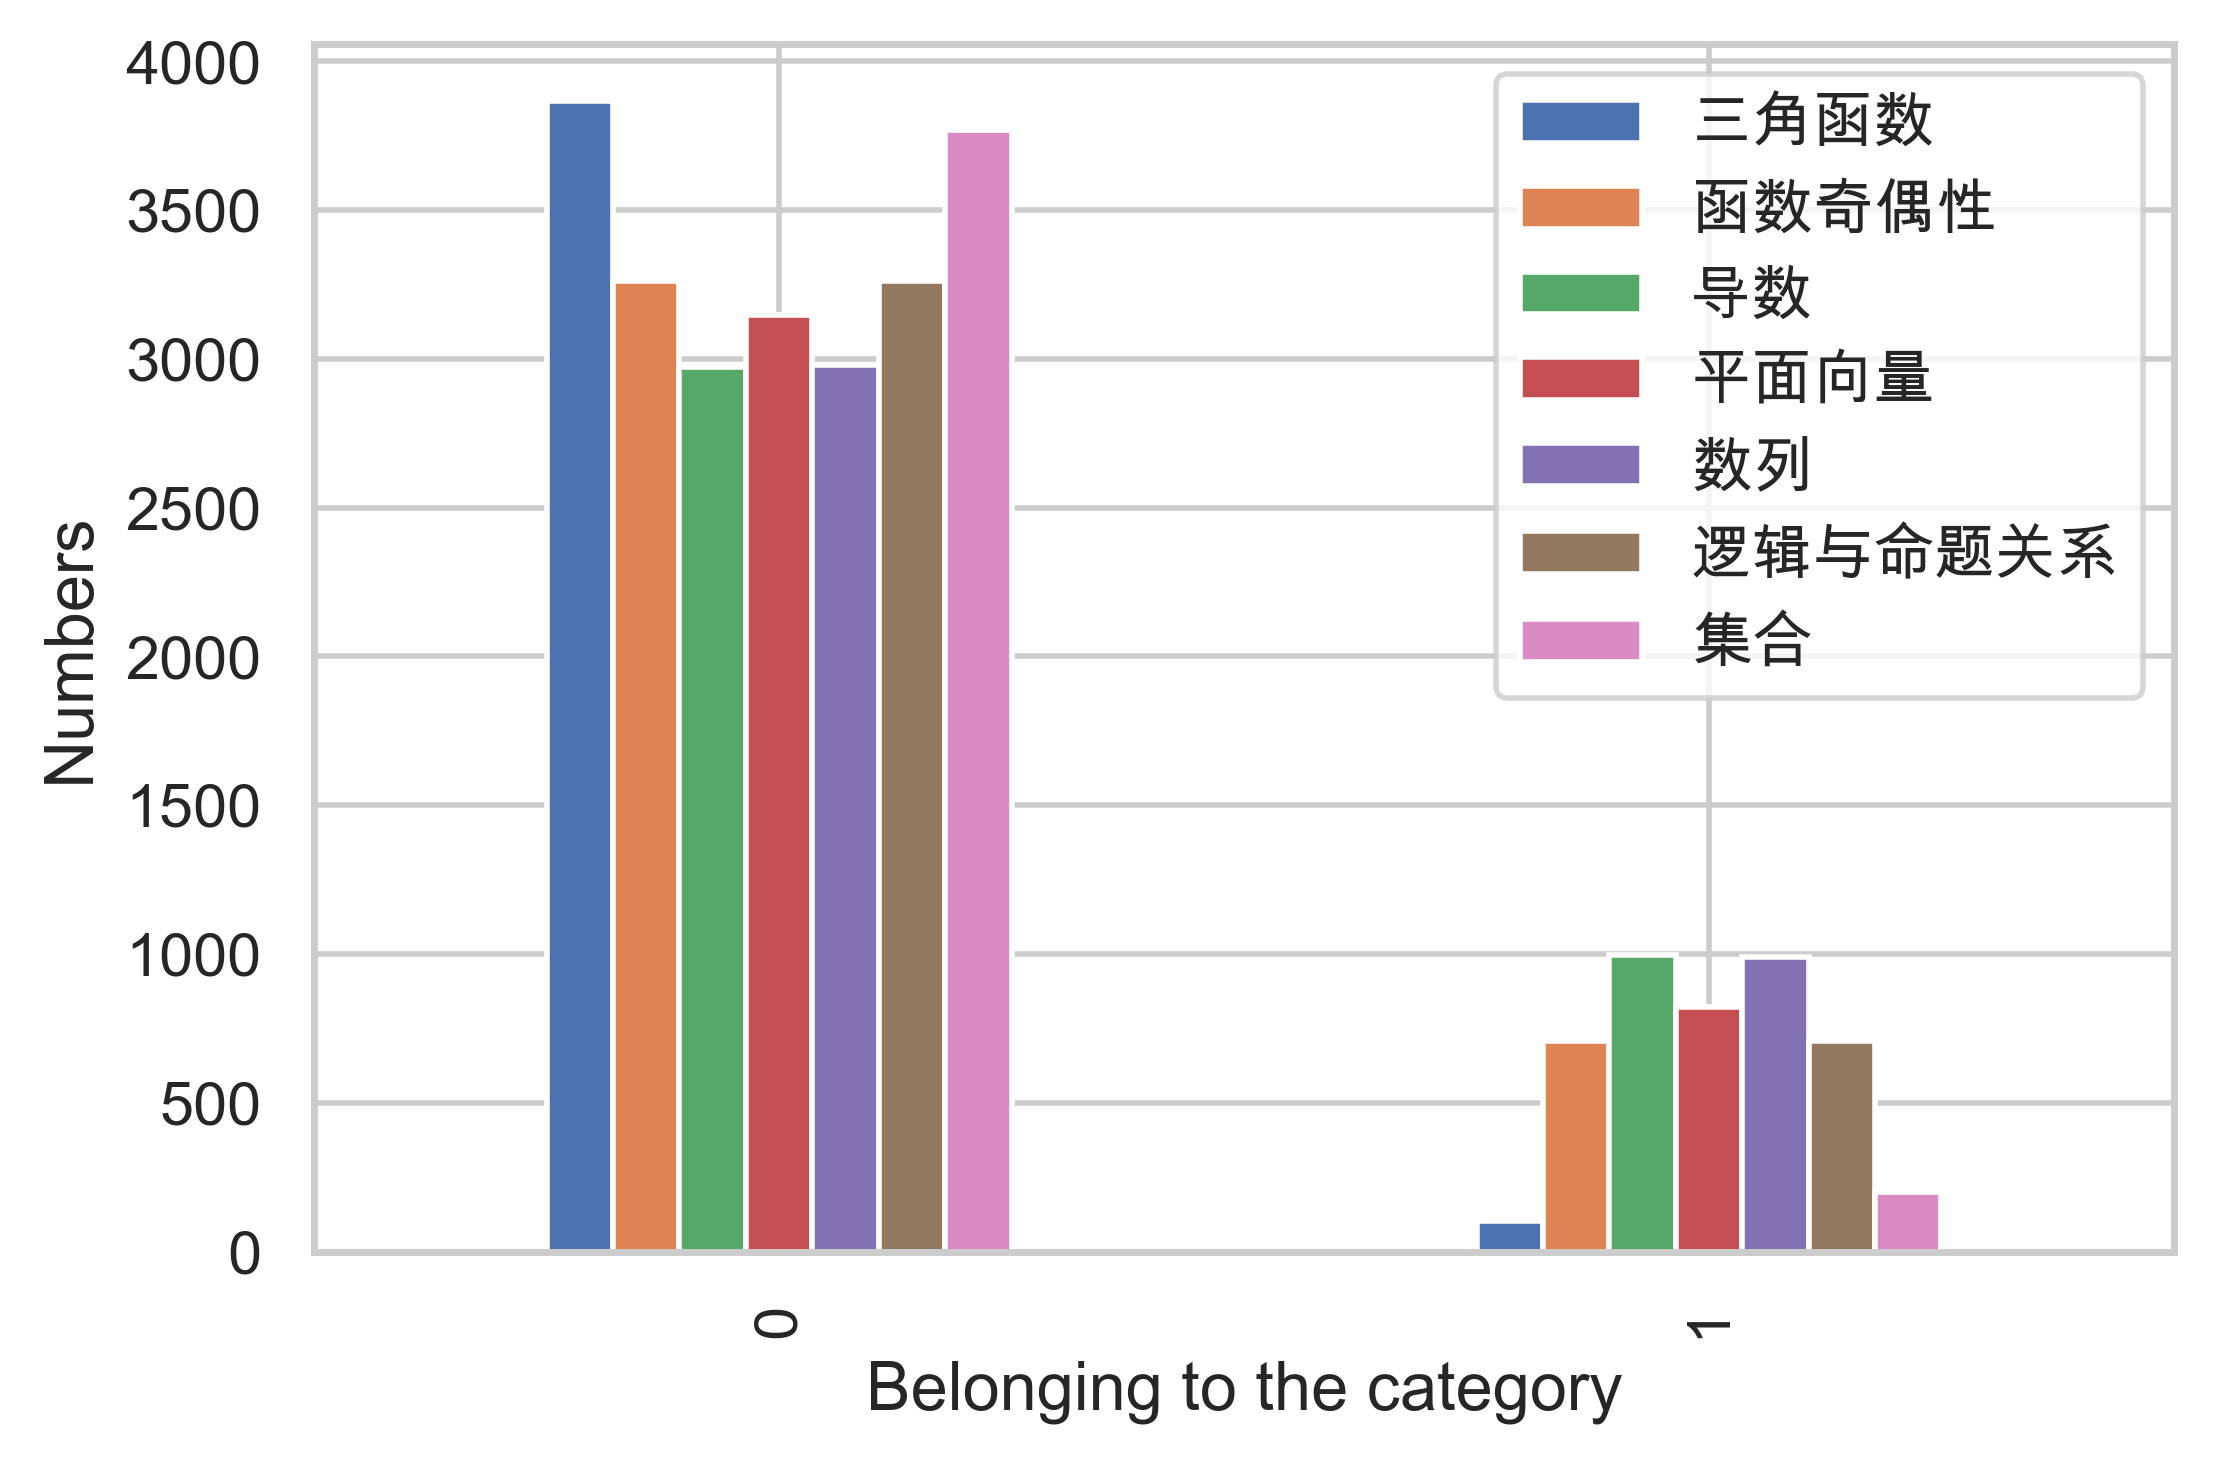
\includegraphics[width=0.85\textwidth]{ch2-data-belonging.png}
    \caption{The distribution of exercise in each category}\label{fig:ch2-data-belonging}
\end{figure}

\begin{figure}[htb]
    \centering
    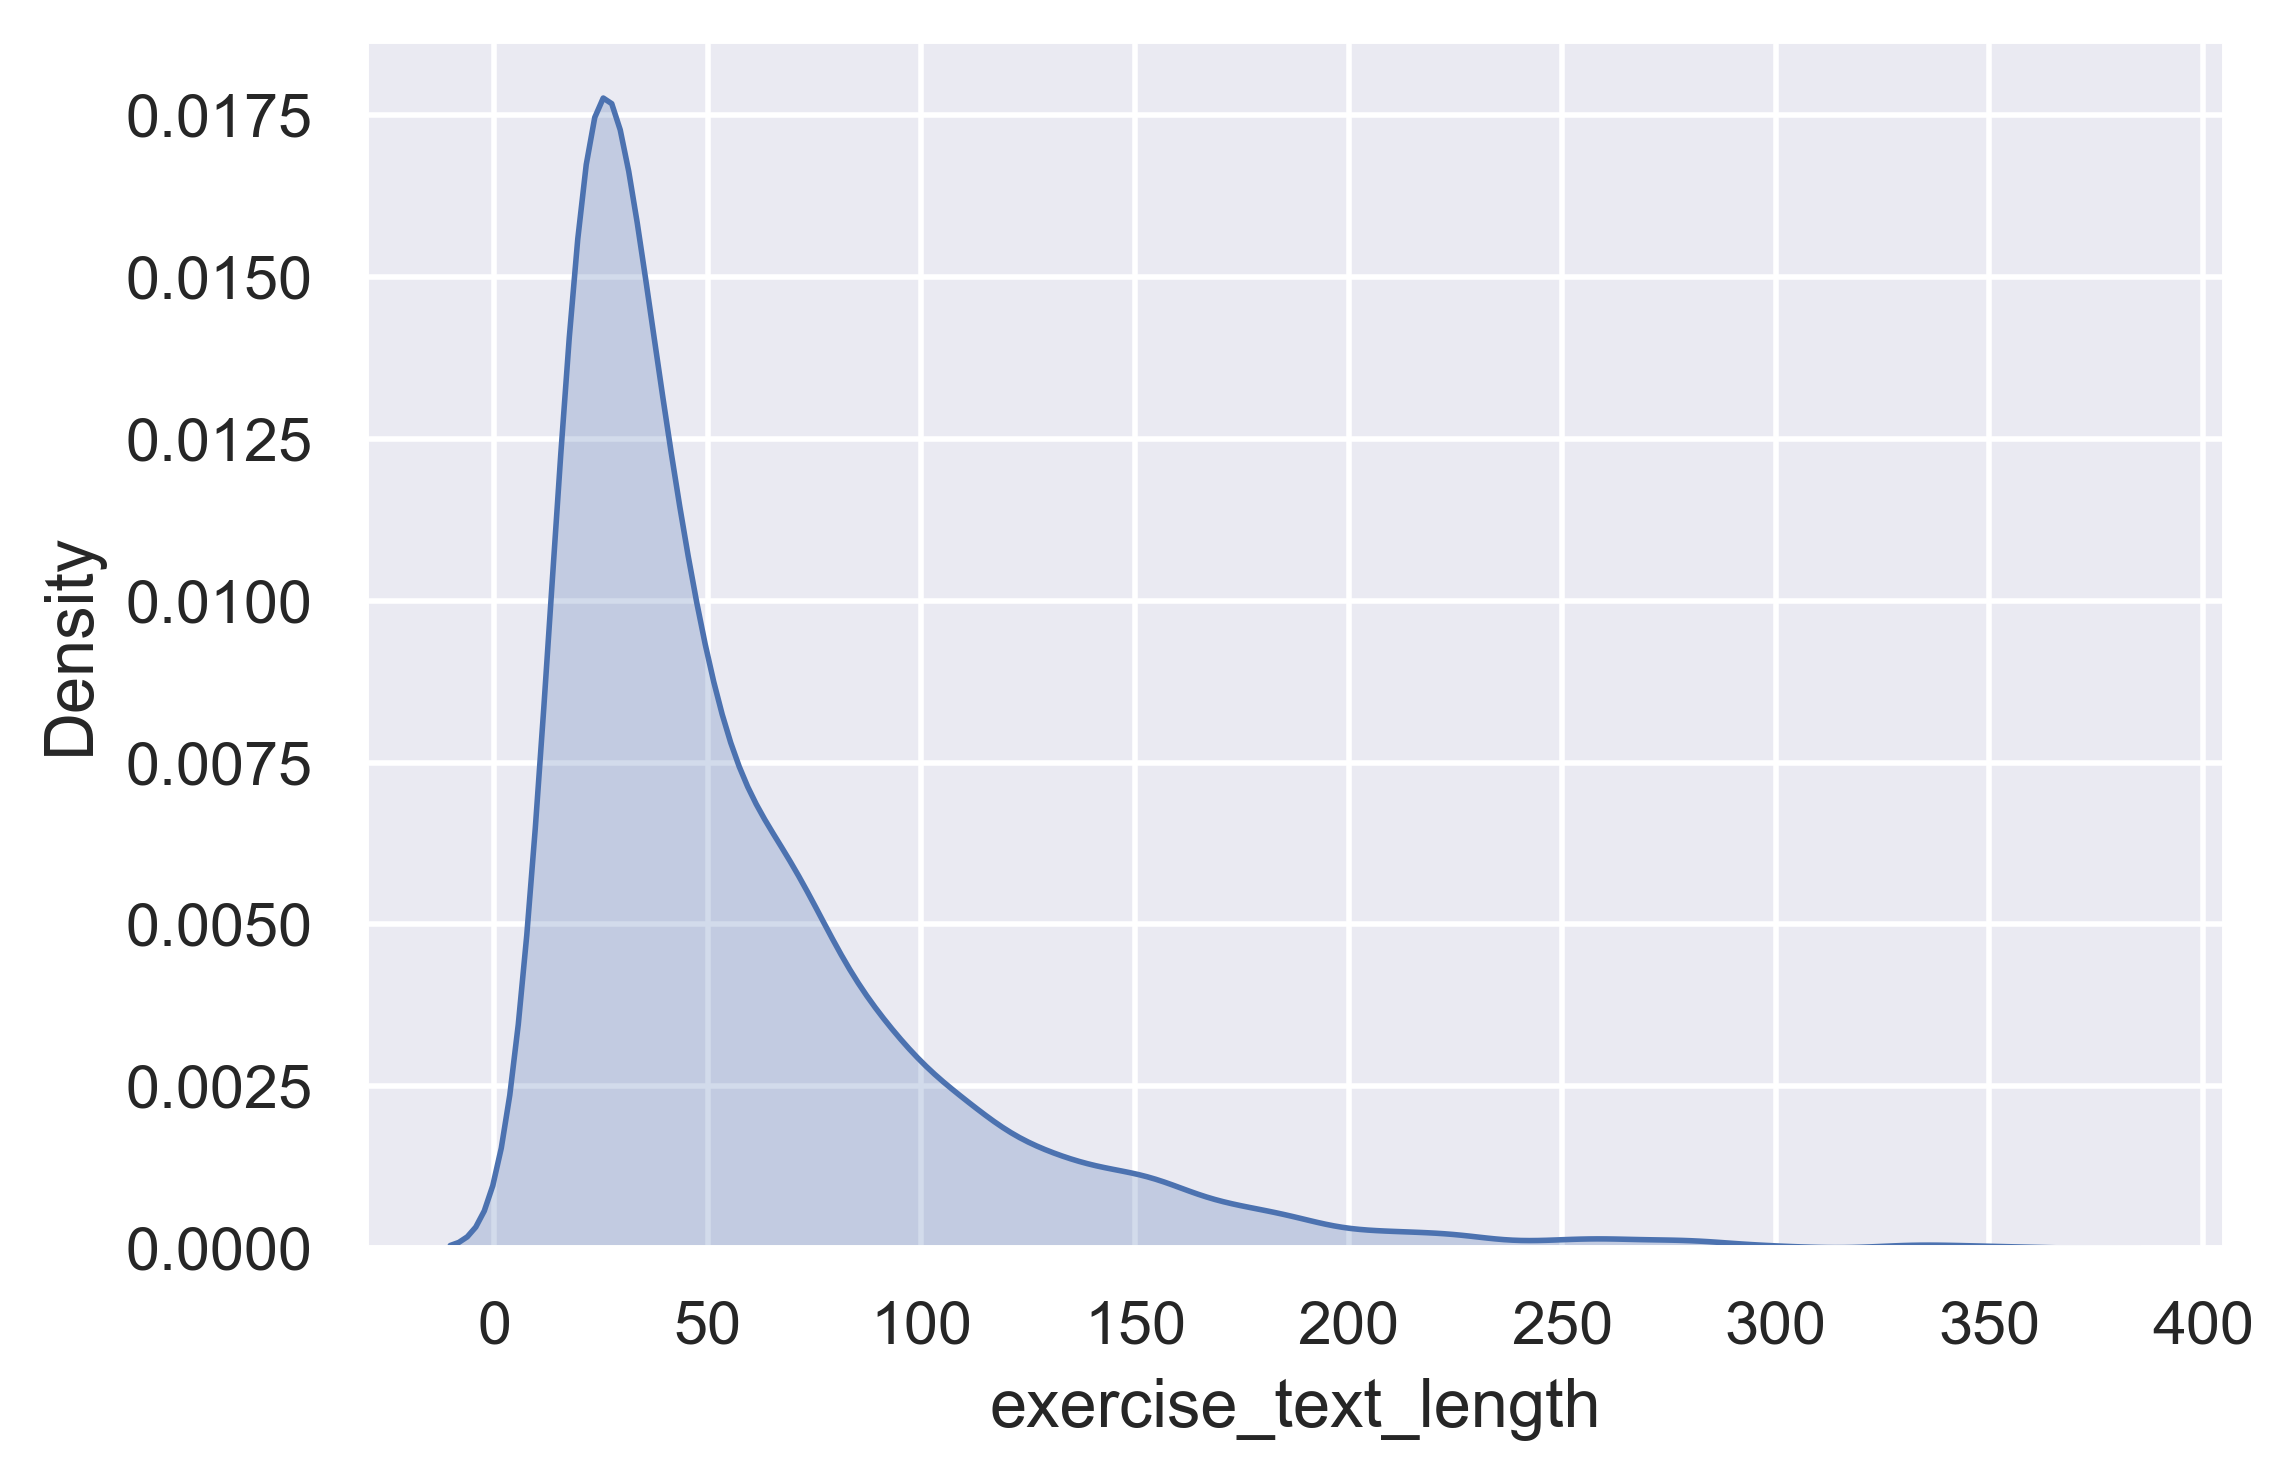
\includegraphics[width=0.85\textwidth]{ch2-data-lendis.png}
    \caption{The distribution of exercise text length}\label{fig:ch2-data-lendis}
\end{figure}

%另外,对于各个类别,可以分析类别间的互相关性,绘制出热力图如图所示。
In addition, for each category, the inter-correlation between the categories can be analyzed and a heat map can be drawn as shown in \figname{\ref{fig:ch2-data-heatmap}}. The results show that some categories in the processed dataset have direct positive correlations and others have negative correlations.
\begin{figure}[htb]
    \centering
    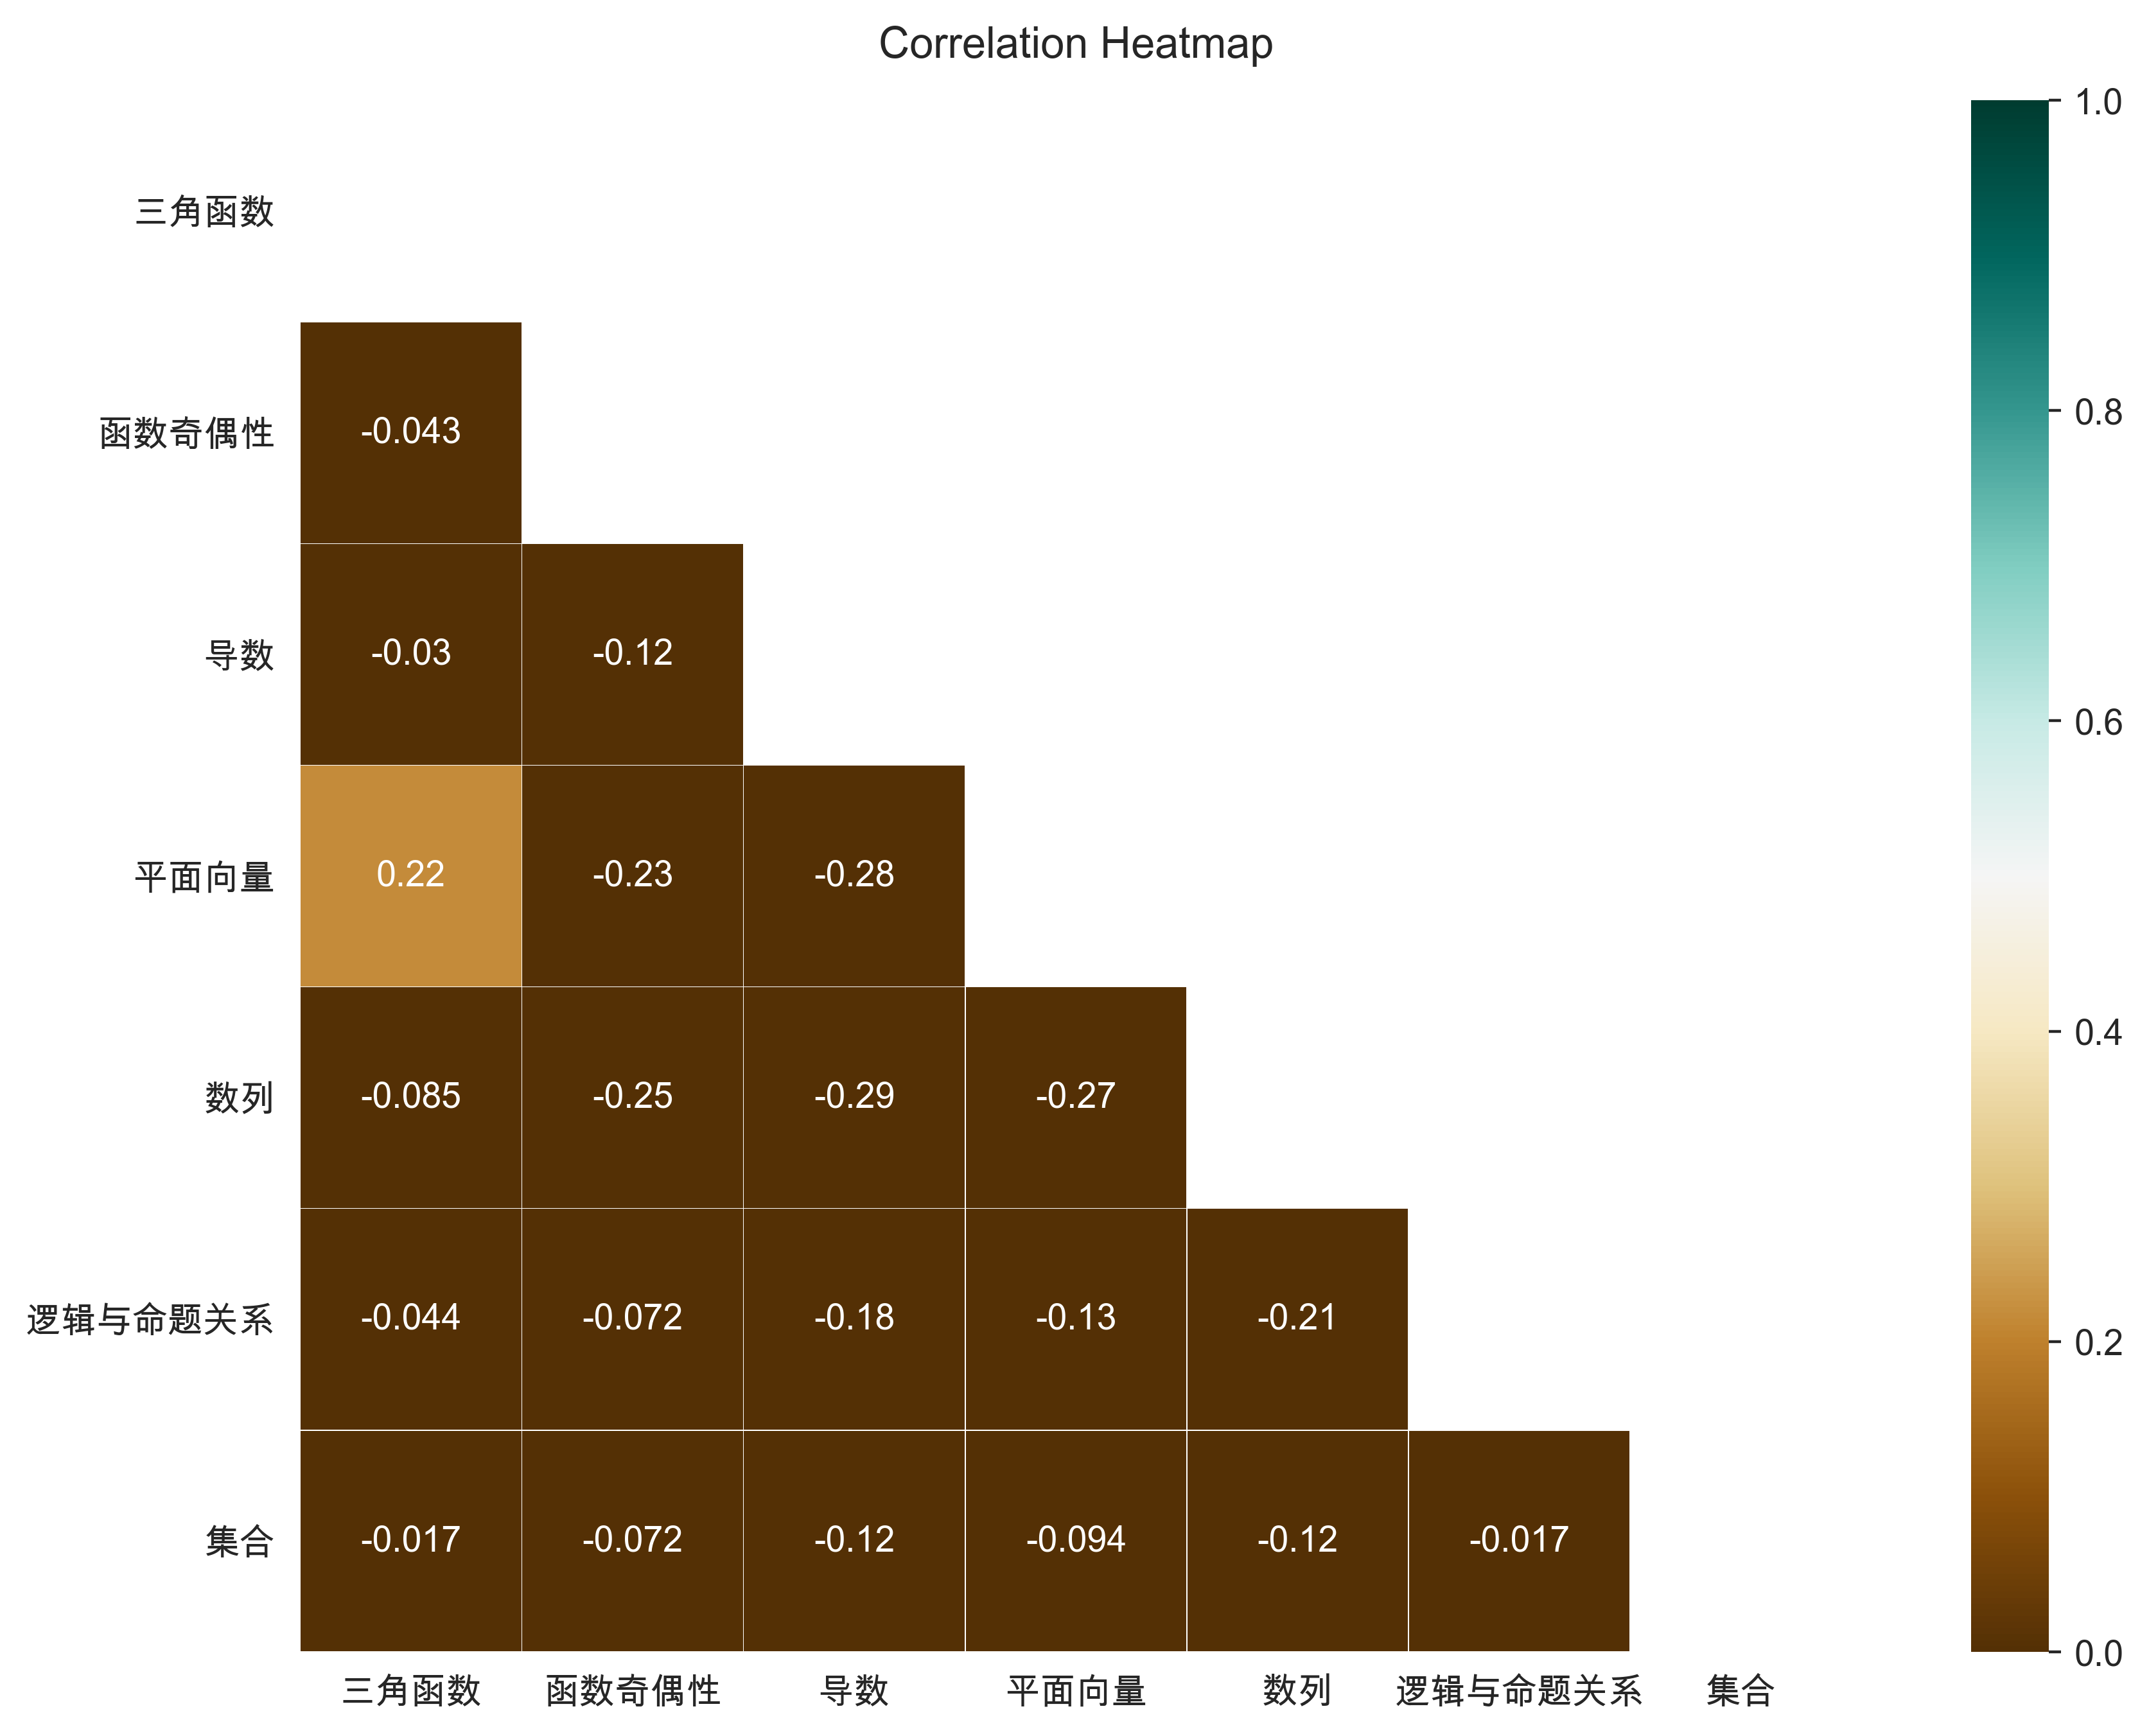
\includegraphics[width=0.85\textwidth]{ch2-data-heatmap.png}
    \caption{The relation heatmap between different categories}\label{fig:ch2-data-heatmap}
\end{figure}



\subsection{Metrics}
%相比于传统学习问题,对多标签数据的标注十分困难,多标签意味着巨大的分类成本。本节的任务中,需要对试题进行多知识点标注,实际上是一个多标签分类问题,则样本维度、数据量、标签维度都会影响标注效果。本节利用了基于标签的评测方法来对提出的试题知识点标注模型进行性能评估。
Compared with common text classification problems, it is hard to label multi-label data, and multi-label means huge classification cost~\cite{zhang2013review}. In the tasks in this section, the test questions need to be labeled with multiple knowledge points. It is a multi-label classification problem. The sample dimension, data volume, and label dimension will all affect the labeling effect. This section uses label-based metrics to evaluate the performance of the proposed test knowledge point labeling model.

%关于多标签分类,考虑到习题的标签之间的关系,本文使用了基于标签的指标来进行模型评估。该指标对每个标签分别进行混淆矩阵指标计算计算出True Positive,False Positive,True Negative和False Negative的样本值。然后计算F1指标值,以此进行多标签指标评估。

Regarding multi-label classification, considering the relationship between the exercises' labels, this thesis uses label-based indicators for model evaluation. The indicator calculates the confusion matrix indicator for each label to calculate the sample values of True Positive (TP), False Positive (FP), True Negative (TN), and False Negative (FN). Then calculate the macro-F1 and micro-F1 metrics for multi-label tagging model performance evaluation.

According to the metrics proposed by Zhou et al.~\cite{zhang2013review}, for the jth label of the ith example in the \(n\) examples, shown in the \eqname{\ref{fml:mlcm}}, where \(x_i\) and \(L_j\) represents the ith exercise and jth label, \(Y_i\) and \(\tilde{Y}_i\) represent the real labels and predicted labels of the ith exercise.

\begin{align}\label{fml:mlcm}
    \begin{split}
        \operatorname{TP}_j & =| \{x_i| L_j\in Y_{i}\wedge L_j \in \tilde{Y}_i , 1\leq i \leq n\}|       \\
        \operatorname{FP}_j & =| \{x_i| L_j\notin Y_{i}\wedge L_j \in \tilde{Y}_i , 1\leq i \leq n\}|    \\
        \operatorname{TN}_j & =| \{x_i| L_j\notin Y_{i}\wedge L_j \notin \tilde{Y}_i , 1\leq i \leq n\}| \\
        \operatorname{FN}_j & =| \{x_i| L_j\in Y_{i}\wedge L_j \notin \tilde{Y}_i , 1\leq i \leq n\}|
    \end{split}
\end{align}

%在混淆矩阵中,Precision为预测正确的正例数据占预测为正例数据的比例,Recall为预测为正例的数据占实际为正例数据的比例。F1值是精确率和召回率的调和均值,它是精确率和召回率的综合评价指标。其计算公式如下:

In the confusion matrix, Precision \(\operatorname{P}\) is the proportion of data with correct predictions to the data that is predicted to be positive, and Recall \(\operatorname{R}\) is the proportions of data with predictions that are positive to the actual data. The \(\operatorname{F1}\) score value is the harmonic mean value of precision rate and recall rate, and it is a comprehensive evaluation index of precision rate and recall rate. The calculation formula is as \eqname{\ref{fml:f1score}}.

\begin{align}\label{fml:f1score}
    \begin{split}
        \operatorname{P}          & =\frac{\operatorname{TP}}{\operatorname{TP}+\operatorname{FP}}    \\
        \operatorname{R}          & =\frac{\operatorname{TP}}{\operatorname{TP}+\operatorname{FN}}    \\
        \operatorname{F1} & = \frac{2}{\frac{1}{\operatorname{P}}+\frac{1}{\operatorname{R}}}
    \end{split}
\end{align}


%micro F1 通过先计算总体的TP,FN和FP的数量,再计算F1, 而macro F1 分别计算每个类别的F1,然后做平均(各类别F1的权重相同)
Similarly, for the multi-label tagging problem, Macro F1 and Micro F1 can be used as the metrics. Micro-F1 first calculates the total number of TP, FN, and FP, and then calculates F1, while Macro-F1 calculates the F1 of each category separately and then averages (the weight of each category F1 is the same). The formula is \eqname{\ref{fml:f1-macro}} and \eqname{\ref{fml:f1-micro}}. The \(c\) is the total number of labels.

\begin{align}
    \operatorname{F1}_{macro} & =\frac{1}{c} \sum_{j=1}^{c} \operatorname{F1}(\operatorname{TP}_{j}, \operatorname{FP}_{j}, \operatorname{TN}_{j}, \operatorname{FN}_{j}) \label{fml:f1-macro}                                  \\
    \operatorname{F1}_{micro} & =\operatorname{F1}(\sum_{j=1}^{c} \operatorname{TP}_{j}, \sum_{j=1}^{c} \operatorname{FP}_{j}, \sum_{j=1}^{c} \operatorname{TN}_{j}, \sum_{j=1}^{c} \operatorname{FN}_{j}) \label{fml:f1-micro}
\end{align}

% 同样的,我们也可以基于样本统计一些指标。例如准确率,海明损失,查全率和F1值。准确率即预测标签完全正确的样本占总体样本的比例,海明损失为预测标签与真是标签的差距的度量指标,Precision和Recall分别代表真阳性样本占真样本的比例和真阳性样本占阳性样本的比例。它 们的计算公式为
Similarly, the statistic of some indicators based on samples can be obtained. For example, the multi-label accuracy rate \(\operatorname{Acc}_{ML}\), multi-label precision rate \(\operatorname{Precision_{ML}}\), multi-label recall rate \(\operatorname{Recall_{ML}}\) and \(\operatorname{F1}_{ML}\) can be calculated. Accuracy is the proportion of samples with completely correct predicted labels in the overall sample. Hamming loss is a measure of the difference between the predicted label and the true label. Precision and Recall represent the proportion of true positive samples in true samples and the proportion of true positive samples in positive samples proportion. Their calculation formulas are \eqname{\ref{fml:subaccuracy}}-{\ref{fml:f1scoreh}}.
\begin{align}
    \operatorname{Acc}_{ML}       & =\frac{1}{n} |\{i|Y_i=\tilde{Y}_i\}| \label{fml:subaccuracy}                                                                              \\
    \operatorname{Precision_{ML}} & =\frac{1}{n} \sum_{i=1}^{n} \frac{|Y_{i} \cap \tilde{Y}_i|}{|\tilde{Y}_i|} \label{fml:Precisionh}                                         \\
    \operatorname{Recall_{ML}}    & =\frac{1}{n} \sum_{i=1}^{n} \frac{|Y_{i} \cap \tilde{Y}_i|}{|Y_{i}|}    \label{fml:Recallh}                                               \\
    \operatorname{F1}_{ML}        & =\frac{2 \cdot \operatorname{Precision} \cdot \operatorname{Recall}}{\operatorname{Precision}+\operatorname{Recall}} \label{fml:f1scoreh}
\end{align}

\subsection{Experiment Settings}
%本模型解决的问题是相关知识点的标注,因此应该在实验中对具有关联知识点的习题分类性能进行评估。
The problem addressed by this model is the labeling of related knowledge points, so the performance of classifying exercises with related knowledge points should be evaluated in the experiment. Therefore this model is trained and will be applied on multi-knowledge point exercises for accuracy, AUC, and multi-classification metrics and compared with the baseline model.

%本实验将训练集和测试集按照3:7的比例划分,并取训练集的1/10作为验证集。
In this experiment, the training and test sets are split from the original dataset by the ratio of 3:7, and one-tenth of the training set is taken as the validation set. All steps of this experiment are run on a stable cloud server environment to ensure the experimental environment's consistency. The running environment are shown in \tblname{{\ref{tbl:ch2-exp-env}}}. Furthermore, there are many adjustable hyperparameters within the model, several critical ones of which are shown in \tblname{\ref{tbl:ch2-hpsetting}}.

% The distribution of the number of exercise knowledge points in this data set is shown in the figure. The number of questions involved in different knowledge points is different. The set of questions involved in knowledge points \(j\) is defined as \(\mathbf{E}_j\). Remember the threshold of the number of occurrences of the knowledge point label \(\tau^{(KP)} \), then the knowledge points of the exercises can be divided according to the frequency of occurrence, i.e., \( \{j|\mathbf{E}_j|>\tau^{(KP)}\} \) and \( \{j||\mathbf{E}_j|\leq\tau^{(KP)} \} \). According to the different thresholds, the model's ability to classify knowledge points frequently and appear sparse can be tested separately.

%在实验中,设定了200,150,100,50,10五组阈值\(\tau^{(KP)} \),将具有标签\(j\)的习题记作\(\mathbb{E}_j\),则可以统计符合要求的标签集\(\mathbb{L}={j||\mathbb{E}_j|\geq\tau^{(KP)}}\)出习题集大小\(|\mathbb{E}_j|\)和题均知识点数\(LAvg_j \)。
% In the experiment, five sets of thresholds of 200, 150, 100, 50, 10 are set \(\tau^{(KP)} \), and the exercises with the label \(j\) are recorded as \(\mathbf{E}_j\), the label set that meets the requirements can be counted as \(\mathbf{L}_\tau^{(KP)}=\{j\mid |\mathbf{E}_j|\geq\tau^{(KP)}\} \), the exercises containing label in \(\mathbf{L}_\tau^{(KP)} \) is denoted as \(\mathbf{E}_\tau^{(KP)} \), within which the average number of knowledge points of the exercise in the set is \(\overline{L}\).

% \begin{table}[htb]
%     \centering
%     \caption{Setting of experiment}\label{tbl:ch2-ex1}
%     \begin{tabular}{cccc}%{cp{2cm}<{\centering}p{2cm}<{\centering}p{2cm}<{\centering}}
%         \toprule
%         \text{\(\tau^{(KP)} \)} & \(|\mathbf{L}_{\tau^{(KP)}}|\) & \(|\mathbf{E}_{\tau^{(KP)}}| \) & \(\overline{L}\) \\
%         \midrule
%         200                     & 2                              & 463                             & 1.21             \\
%         100                     & 22                             & 1376                            & 1.55             \\
%         50                      & 29                             & 2237                            & 1.42             \\
%         10                      & 57                             & 3158                            & 1.35             \\
%         \bottomrule
%     \end{tabular}
% \end{table}


\begin{table}[htb]
    \caption{Experiment running environment}\label{tbl:ch2-exp-env}
    \centering
    \begin{tabular}{l c}
        \toprule
        Software/Hardware & Configuration   \\
        \midrule
        CPU               & Xeon Gold 6139  \\
        GPU               & Tesla V100      \\
        VRAM              & 16G             \\
        Operating System  & Ubuntu 18.04    \\
        Python            & 3.8.6           \\
        PyTorch           & 1.8.0           \\
        GPU Driver        & Cuda11.2/cudnn8 \\
        \bottomrule
    \end{tabular}
\end{table}



\begin{table}[htb]
    \caption{Hyperparameter settings of recommendation model}\label{tbl:ch2-hpsetting}
    \centering
    \begin{tabular}{l c c}
        \toprule
        Hyperparameter            & Value \\
        \midrule
        Dimension of hidden layer & 64    \\
        Number of GCN Layers      & 2     \\
        Max text length           & 128   \\
        Optimizer                 & Adam  \\
        Learning rate             & 0.001 \\
        Number of classes         & 7     \\
        Batch size                & 32    \\
        Embed size                & 100   \\
        Training epochs           & 20    \\
        \midrule
        \bottomrule
    \end{tabular}
\end{table}

%本实验中,定义了一个GCN架构用于学习知识点间关联,该架构包含两层GCN层,其维度分别为512和1024。每个节点采用256维word2vec来训练标签文本得到标签embedding表示。对于标签correlation阈值\tau则分别设置为多个值来进行模型性能判定。

% In this experiment, a GCN architecture is defined to learn the association between knowledge points. The architecture contains two GCN layers with dimensions of 512 and 1024, respectively. Each node uses 256-dimensional word2vec to train the label text to obtain the label embedding representation. The tag correlation threshold \(\tau \) is set to multiple values to determine the model performance.

% The running environment is Ubuntu 20.04, TensorFlow 2.23, Python 3.8.6, and the hardware is equipped with a Tesla V100 computing card. For each Baseline model, five rounds of calculation are performed, the maximum positive deviation and the minimum negative deviation are discarded, and the average value is recorded.


% \subsubsection{Data Prepartion}
% %本节数据获取的方式为爬虫,因此获得的原始数据为大量非结构化的带有不规范数学符号的习题,这些符号难以被BERT模型处理,会带来误差,因此在预处理的过程中,会将无法识别的字符进行替换。另外还有大量的无意义文本,此外,由于部分习题知识点标注不全,因此需要人工协助标注知识点。
\subsection{Baselines}
% In the algorithm, the binary relation method (BR), the multi-label KN algorithm (ML-KNN) are selected as the comparison algorithm, and the experimental training set test set division ratio, which is 1:1.
% 目前,已经有一些进行文本标签标注的算法模型,为了验证本文提出算法的有效性,将与下列的算法进行比较,作为baseline指标。
This section's study focuses on a multi-label text classification task, so several more popular text classification models are used as baseline models. Some existing text classification models are selected experimentally to compare with the proposed model, and the performance is compared with the proposed model on the selected experimental evaluation metrics and the same dataset. There are already some algorithm models for labeling text, which are set as the baseline models for comparison to verify the effectiveness of the proposed algorithm.
\begin{itemize}
    \item Bi-LSTM+Attention~\cite{zhou2016attention}: the model consists of an Embedding layer, a bi-directional LSTM layer, and an Attention layer. The text is passed through the Embedding layer to generate the Embedding vector, the LSTM to compute the higher-order sentence vector, the Attention layer to weight the sentence vector, and the final output layer to output the predicted labels.
    \item fastText~\cite{joulin-etal-2017-bag}: Facebook proposes the fastText model in 2017. The fastText accelerated training and can be applied to text classification tasks, and it contains input, hidden, and output layers. The method is actually a weighted sum of the word vectors of the sentences as sentence vectors, using softmax classification.
    \item TextCNN~\cite{guo2019improving}: Kim et al.\ adapted the CNN to the text classification task by improving it in 2014~\cite{kim-2014-convolutional}. It contains parts such as the convolutional layer, max-pooling layer, and output layer. The principle is to extract higher-order features of text by multiple convolutional kernels, and it can introduce pre-trained word vectors to improve the performance.

\end{itemize}

\subsection{Model Training}
%训练的损失函数图和准确率图如图所示。在训练的过程中,当遇到更好的验证准确率时,将会保留模型参数,当训练结束好保存的模型即是最优模型,它将会应用于测试集进行模型性能验证。
The training and validation loss plot are shown in \figname{\ref{fig:ch2-training-loss}} and the accuracy plots are shown in \figname{\ref{fig:ch2-training-acc}}. During the training process, when better validation accuracy is encountered, the model parameters will be preserved, and when the training is finished, the saved model is the optimal model, which will be applied to the test set for model performance validation. According to the training graph, it can be concluded that the model converges after about 15 epochs of training.
\begin{figure}[htb]
    \centering
    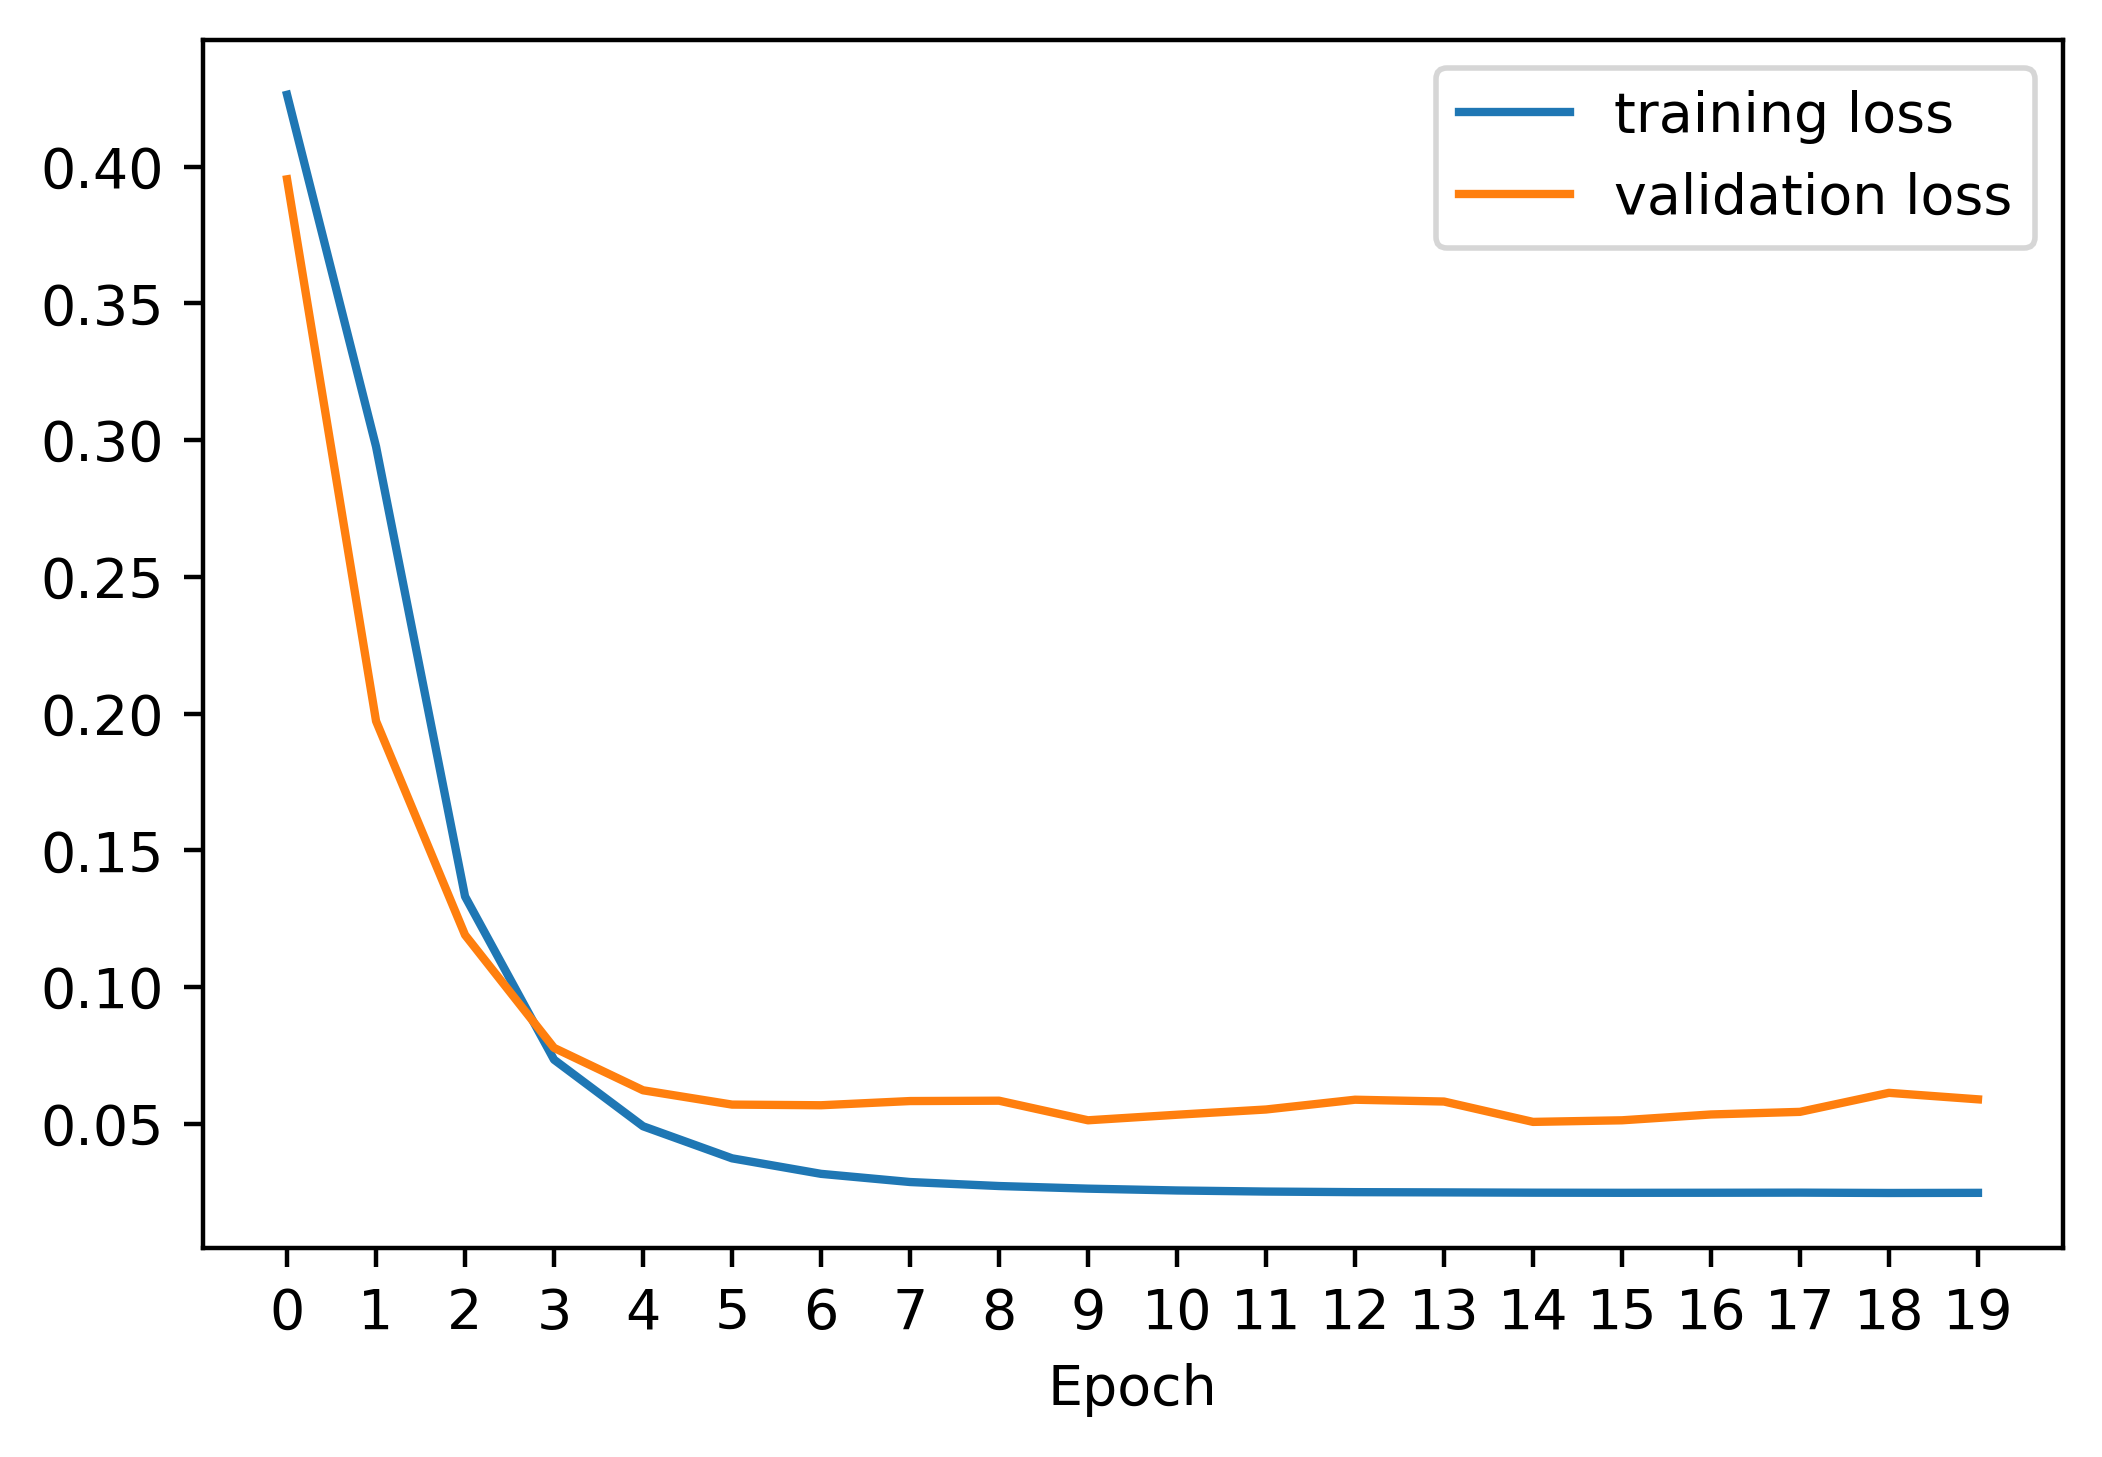
\includegraphics[width=0.85\textwidth]{ch2-training-loss.png}
    \caption{The training and validation loss plot of model}\label{fig:ch2-training-loss}
\end{figure}

\begin{figure}[htb]
    \centering
    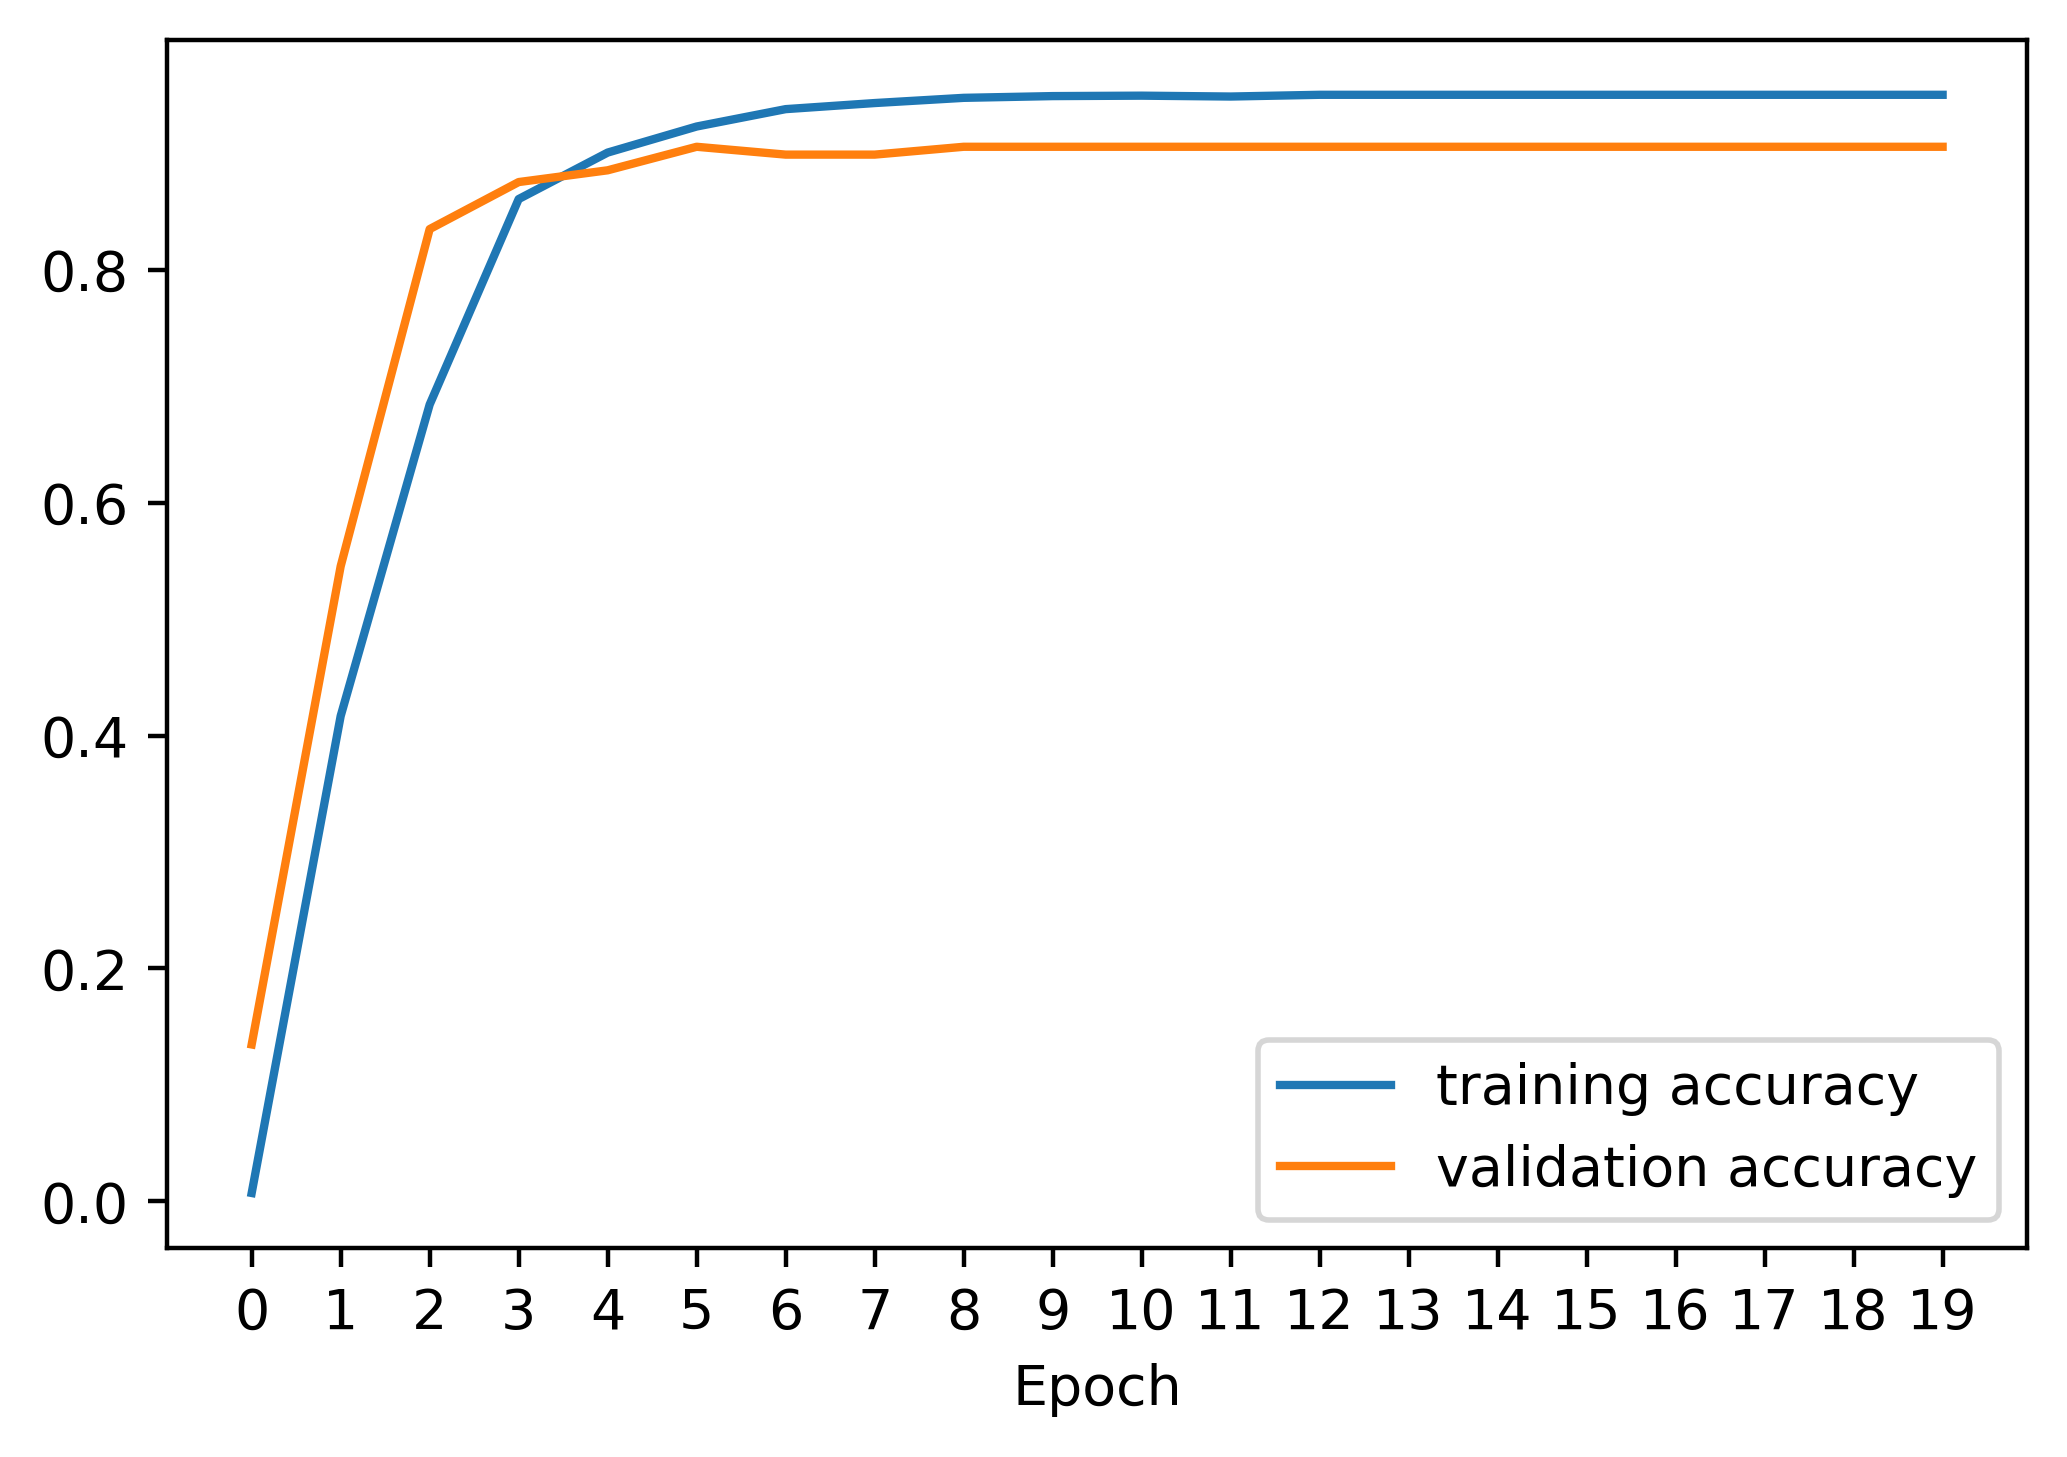
\includegraphics[width=0.85\textwidth]{ch2-training-acc.png}
    \caption{The training and validation acc plot of model}\label{fig:ch2-training-acc}
\end{figure}

\subsection{Result and Analysis}
In the experimental comparison for each of the other baseline models, three experiments were conducted, and the average of the experimental results was taken as the performance parameter of the baseline model and compared with the proposed model. The comparison experiment results are divided into the performance comparison of the baseline models shown in \tblname{\ref{tbl:ch2-result-bsline1}}. The results show that the proposed model outperforms the baseline model in all the multi-label classification metrics, so the present model achieves the intended design goal. Further, the classification details of the model for each category are shown in \tblname{\ref{tbl:ch2-result-detail}}.

\begin{table}[htbp!]
    \caption{Performance comparison between baseline and proposed models}\label{tbl:ch2-result-bsline1}
    \centering
    \begin{tabular}{ccccc}
        \toprule
        Metrics           & \(\operatorname{F1}_{macro}\) & \(\operatorname{F1}_{micro}\) & \(\operatorname{Acc}_{ML}\) & \(\operatorname{F1}_{ML}\) \\
        \midrule
        BiLSTM+Attention  & 0.824                         & 0.924                         & 0.874                       & 0.926                      \\
        fastText          & 0.846                         & 0.922                         & 0.854                       & 0.916                      \\
        TextCNN           & 0.761                         & 0.923                         & 0.857                       & 0.917                      \\
        \textbf{Proposed} & \textbf{0.912}                & \textbf{0.932}                & \textbf{0.888}              & \textbf{0.937}             \\
        \bottomrule
    \end{tabular}
\end{table}

As can be seen from the \tblname{\ref{tbl:ch2-result-detail}}, the performance of the models proposed in this chapter is better for exercises that occur more frequently than those that occur less frequently. As the frequency of knowledge points decreases and the difficulty of classification increases, the model shows performance degradation. This is because the model is prone to overfitting when the exercises' sample size is small, leading to the degradation of the model prediction performance. The problem can be solved by increasing the sample size and optimizing the data quality.

\begin{table}[htbp!]
    \caption{Classification report of proposed model}\label{tbl:ch2-result-detail}
    \centering
    \begin{tabular}{ccccc}
        \toprule
        Class          & Precision & Recall & F1 Score & Support \\
        \midrule
        三角函数       & 0.957     & 0.710  & 0.815    & 31      \\
        函数奇偶性     & 0.946     & 0.930  & 0.938    & 187     \\
        导数           & 0.918     & 0.866  & 0.892    & 247     \\
        平面向量       & 0.942     & 0.961  & 0.951    & 204     \\
        数列           & 0.996     & 0.971  & 0.983    & 243     \\
        逻辑与命题关系 & 0.958     & 0.883  & 0.919    & 180     \\
        集合           & 0.907     & 0.867  & 0.886    & 45      \\
        \midrule
        Micro avg      & 0.951     & 0.915  & 0.932    & 1137    \\
        Macro avg      & 0.946     & 0.884  & 0.912    & 1137    \\
        Weighted avg   & 0.951     & 0.915  & 0.932    & 1137    \\
        Samples avg    & 0.951     & 0.935  & 0.937    & 1137    \\
        \bottomrule
    \end{tabular}
\end{table}



% \begin{table}
%     \centering
%     \caption{Result comparison (\(\tau^{(KP)}=100 \))}\label{tbl:bsline2}
%     \begin{tabular}{cccccccc}
%         \toprule
%         Metrics  & \(\operatorname{F1}_{macro}\) & \(\operatorname{F1}_{micro}\) & \(\operatorname{Acc}_{ML}\) & \(\operatorname{HmLoss}\) & \(\operatorname{F1}_{ML}\) \\
%         \midrule
%         NB       & 71.2                          & 72.1                          & 67.2                        & 16.2                      & 71.8                       \\
%         ML-KNN   & 73.2                          & 72.3                          & 69.1                        & 15.9                      & 74.7                       \\
%         CNN+BERT & 74.4                          & 74.6                          & 72.3                        & 13.1                      & 75.1                       \\
%         Proposed & \textbf{75.5}                 & \textbf{75.7}                 & \textbf{73.1}               & \textbf{12.7}             & \textbf{74.9}              \\
%         \bottomrule
%     \end{tabular}
% \end{table}

% \begin{table}
%     \centering
%     \caption{Result comparison (\(\tau^{(KP)}=50 \))}\label{tbl:bsline3}
%     \begin{tabular}{cccccccc}
%         \toprule
%         Metrics      & \(\operatorname{F1}_{macro}\) & \(\operatorname{F1}_{micro}\) & \(\operatorname{Acc}_{ML}\) & \(\operatorname{HmLoss}\) & \(\operatorname{F1}_{ML}\) \\
%         \midrule
%         NB           & 52.3                          & 53.0                          & 42.1                        & 9.2                       & 51.9                       \\
%         ML-KNN       & 44.2                          & 43.9                          & 23.5                        & 10.1                      & 42.1                       \\
%         CNN+word2vec & 56.1                          & \textbf{57.3}                 & 46.2                        & 8.2                       & 56.5                       \\
%         CNN+BERT     & 56.2                          & 56.8                          & \textbf{47.0}               & \textbf{8.1}              & 56.1                       \\
%         Proposed     & \textbf{57.1}                 & 57.2                          & 45.2                        & 8.6                       & \textbf{57.5}              \\
%         \bottomrule
%     \end{tabular}
% \end{table}

% \begin{table}
%     \centering
%     \caption{Result comparison (\(\tau^{(KP)}=10 \))}\label{tbl:bsline4}
%     \begin{tabular}{cccccccc}
%         \toprule
%         Metrics  & \(\operatorname{F1}_{macro}\) & \(\operatorname{F1}_{micro}\) & \(\operatorname{Acc}_{ML}\) & \(\operatorname{HmLoss}\) & \(\operatorname{F1}_{ML}\) \\
%         \midrule
%         NB       & 36.5                          & 37.1                          & 26.1                        & 4.2                       & 36.5                       \\
%         ML-KNN   & 30.1                          & 32.1                          & 29.1                        & 3.6                       & 32.5                       \\
%         CNN+BERT & 36.9                          & \textbf{38.6}                 & \textbf{38.6}               & \textbf{3.5}              & 37.5                       \\
%         Proposed & \textbf{37.1}                 & 38.3                          & 35.4                        & 3.8                       & \textbf{38.6}              \\
%         \bottomrule
%     \end{tabular}
% \end{table}

%从表中可以看出,本文提出的模型在出现频次较高的习题训练机上的性能表现强于Baseline模型。随着知识点出现频率的降低,分类的难度增大,所有模型都出现了性能退化现象。其中的原因是模型对于出现较少的标签无法进行有效的信息抓取,从而产生的误差增大。总体而言,在F1-Score参数和较为严格的子集准确率指标上,本文提出的模型都取得了最优或较优的性能表现。当习题标签频次出现次数非常低时,几乎所有的模型都无法取得较好的结果,这是因为由于习题标签的频次分布不均匀,少量冷门标签无法很好地标注,导致模型训练出现了过拟合现象从而影响标注表现。为了解决该问题,可以通过用更大和知识点出现频次较为平均的习题集作为训练集来优化模型预测性能表现。

% It can be seen from the table that the performance of the model proposed in this thesis is stronger than the baseline model on the exercise training machine with a higher frequency. As the frequency of knowledge points decreases, classification difficulty increases and performance degradation occurs in all models. The reason is that the model cannot effectively capture information for fewer tags, resulting in increased errors. In general, the model proposed in this thesis has achieved the best or better performance in terms of F1-Score parameters and stricter subset accuracy indicators. When the problem labels' frequency is shallow, almost all models cannot achieve good results. This is because due to the uneven frequency distribution of the problem labels, a small number of unpopular labels cannot be well labeled, resulting in over-fitting in model training. This phenomenon affects labeling performance. In order to solve this problem, the model prediction performance can be optimized by using a larger set of exercises with a more average frequency of knowledge points than the training set.

% From the experimental results, it can be seen that, compared with the binary relation method, the multi-label KNN algorithm, and the classifier chain method, the multi-knowledge point labeling method based on ensemble learning proposed in this thesis has achieved better results under different knowledge point labels. In multi-label classification, the evaluation of more stringent indicators—subset accuracy-this thesis's method is always significantly better than the other three methods. Screening the base classifiers with relatively good performance and integrating their results through the majority voting method compensated for each base classifier's disadvantages and obtained good results. However, as the tag frequency threshold decreases, the number of knowledge points gradually increases, and the difficulty of multi-label classification becomes more and more difficult. One of the reasons is that the knowledge points actually contained in a test question is not completely consistent with the knowledge points that the teacher investigates. As shown in Table 7, in the first three questions, there is no ``arithmetic sequence'' in the original manually labeled knowledge points, but the content of the test questions contains the term ``arithmetic sequence''. Questions 4 and 5 The knowledge point is ``arithmetic sequence'', and there is also ``arithmetic sequence'' in the question stem. Therefore, when using the trained model to predict the first three questions, the ``arithmetic sequence'' will be marked as the knowledge point of this question. It is more difficult to further determine the knowledge points of examination questions and the knowledge points contained in the questions based on the existing data. The second reason is that due to the uneven distribution of knowledge points, many knowledge points do not have enough test data for learning, which makes it difficult to predict the knowledge points in the pre-test questions.


\section{Summary}
%在习题推荐系统中,有数量众多的知识点标签缺失的习题,为了满足自适应学习系统的要求,需要对习题进行知识点标注,但人工标注成本较高,效率较低。因此, 自动标注试题知识点成为了亟待解决的问题。本章提出了一个基于图卷积神经网络和基于注意力机制的Bi-LSTM文本挖掘模型的习题多知识点标注模型。经过对实验数据集的验证,取得了相对现有模型的较好的知识点标注效果。

%本章的贡献有以下几点:
%(1)通过图神经网络表征知识点间的关系,从而可以挖掘出原文本中隐藏的知识点标签,给现有的模型提供了知识点标签联想推理功能。
%(2)通过设计知识点间关联函数,对知识点间依赖进行建模,并取得了较好的性能表现。
%(3)验证了低知识点标签频次对于多标签分类模型会产生过拟合现象,从而造成性能退化,为了解决该问题,可以通过平均训练数据集标签频次来解决。

%习题知识点标注是推荐系统的第一步,经过标注的习题可以作为知识追踪模型的输入,从而追踪学生的知识状态,也可以作为推荐系统的输入特征来完成基于知识点的习题推荐。

In the exercise recommendation system, there are a large number of exercises with missing knowledge point labels. It is necessary to label the exercises to meet the adaptive learning system's requirements, while manual labeling is high cost and low efficiency. Therefore, automatic marking of knowledge points of test questions is a critical problem to be solved. This chapter proposes a multi-knowledge point labeling model for exercises based on GCN and Bi-LSTM text mining model based on the attention mechanism. For the proposed model, a better knowledge point labeling performance than existing models has been achieved after verifying the experimental data set.

The contributions of this chapter are as follows:
\begin{enumerate}
    \item The relationship between knowledge points is modeled by a graph neural network, which can expose the hidden knowledge point labels in the original text and provide the existing model with the latent knowledge point reasoning capability.
    \item By designing the correlation function between the knowledge points, the dependence between the knowledge points is modeled based on knowledge points' co-existence in the same exercise.
    \item The proposed model achieved better performance than baseline models in multi knowledge labeling task.
\end{enumerate}

The labeling of exercise knowledge points is the first step of the recommendation system. The labeled exercises can be used as the input of the knowledge tracing model to track students' knowledge state and can also be adopted as the recommendation system's input feature to recommend exercises based on knowledge points.

